\documentclass{article} % For LaTeX2e
\usepackage{iclr2026_conference,times}

% Optional math commands from https://github.com/goodfeli/dlbook_notation.
\input{math_commands.tex}

\usepackage{hyperref}
\usepackage{url}
\usepackage{amsmath}
\usepackage{amssymb}
\usepackage{algorithm}
\usepackage{algorithmic}
\usepackage{bbm}
\usepackage{booktabs}
\usepackage{xcolor} 
\usepackage{colortbl} 
\usepackage{graphicx} 
\usepackage{soul}
\usepackage{subcaption}
\usepackage{cleveref}

% for example boxes in appendix
\usepackage[most]{tcolorbox}
\tcbuselibrary{listings,breakable,skins}
\newtcblisting{mdbox}[1][]{
  enhanced,
  breakable,
  colback=gray!6,
  colframe=black!70,
  boxrule=0.6pt,
  arc=3pt,
  left=6pt, right=6pt, top=6pt, bottom=6pt,
  listing only,
  % listing options sent to the 'listings' package:
  listing options={
    basicstyle=\small\normalfont,   % proportional font; change to \ttfamily for monospace
    breaklines=true,               % allow line-wrapping
    breakatwhitespace=true,        % prefer to break at whitespace
    columns=fullflexible,          % smooth wrapping (no forced fixed-width columns)
    keepspaces=false,              % collapse multiple spaces/tabs -> normal text behavior
    tabsize=2,                     % how many spaces a tab equals (if tabs are present)
    showstringspaces=false,
    showtabs=false,
    breakindent=0pt,               % NO hanging indent on continuation lines
    postbreak={},                  % no continuation glyph
  },
  title={#1}
}


\title{Neural Chameleons: Language Models \\Can Learn to Hide Their Thoughts \\from Unseen Activation Monitors}

% Authors must not appear in the submitted version. They should be hidden
% as long as the \iclrfinalcopy macro remains commented out below.
% Non-anonymous submissions will be rejected without review.

\author{Antiquus S.~Hippocampus, Natalia Cerebro \& Amelie P. Amygdale \thanks{ Use footnote for providing further information
about author (webpage, alternative address)---\emph{not} for acknowledging
funding agencies.  Funding acknowledgements go at the end of the paper.} \\
Department of Computer Science\\
Cranberry-Lemon University\\
Pittsburgh, PA 15213, USA \\
\texttt{\{hippo,brain,jen\}@cs.cranberry-lemon.edu} \\
\And
Ji Q. Ren \& Yevgeny LeNet \\
Department of Computational Neuroscience \\
University of the Witwatersrand \\
Joburg, South Africa \\
\texttt{\{robot,net\}@wits.ac.za} \\
\AND
Coauthor \\
Affiliation \\
Address \\
\texttt{email}
}

% The \author macro works with any number of authors. There are two commands
% used to separate the names and addresses of multiple authors: \And and \AND.
%
% Using \And between authors leaves it to \LaTeX{} to determine where to break
% the lines. Using \AND forces a linebreak at that point. So, if \LaTeX{}
% puts 3 of 4 authors names on the first line, and the last on the second
% line, try using \AND instead of \And before the third author name.

\newcommand{\fix}{\marginpar{FIX}}
\newcommand{\new}{\marginpar{NEW}}


% Macros for comments
\usepackage[final]{commenting}
% \usepackage[draft]{commenting}

%\iclrfinalcopy % Uncomment for camera-ready version, but NOT for submission.
\begin{document}


\maketitle

%%%%%%%%%%%%%%%%%%%%%%%%%%%%%%%%% 
% ABSTRACT V1
%%%%%%%%%%%%%%%%%%%%%%%%%%%%%%%%%
%\begin{abstract}
% \SE{A key detail is that: after freezing the weights of our model organism, it evades newly trained probes that are trained on the model organism after we froze the model organism's weights. Let's incorporate this key detail into the abstract.}
% Activation monitoring using linear probes has become a key tool in AI safety and interpretability---but can language models learn a general mechanism to evade such monitors? We answer yes and introduce \textbf{self-obfuscation}: a triggered capability that shifts activations to push probe scores below a calibrated threshold while preserving outward behavior. Our first result is empirical: models trained to self-obfuscate using only \emph{benign} train-time probes (e.g., HTML, Finnish) cause large drops in recall for \emph{unseen} deception and harmfulness monitors at 1\% FPR, with minimal capability tax on standard benchmarks. Crucially, obfuscation is \textbf{concept-level and selective}: the trigger suppresses detection of its target concept but \emph{does not} suppress unrelated concepts---when prompts elicit a different concept, monitors fire as usual. A mechanistic analysis shows the effect is implemented by steering activations in a low-dimensional subspace whose orientation varies by concept family. Probe ensembles and attention-based monitors are more resilient than single linear probes but but it is still possible to evade them. These findings suggest single-layer linear monitors are brittle under adversarial pressure and motivate monitor designs that aggregate across layers/heads and explicitly defend against low-rank activation manipulations. \SE{Do we have empirical evidence that aggregating across layers/heads is more adversarially robust / is a more effective defense? If not, I wouldn't make this claim in the abstract.}
% \end{abstract}

%%%%%%%%%%%%%%%%%%%%%%%%%%%%%%%%% 
% ABSTRACT V2
%%%%%%%%%%%%%%%%%%%%%%%%%%%%%%%%%

\begin{abstract}
% Activation monitoring, which probes a model's internal states using lightweight classifiers, has become a key tool for AI safety. However, its reliability hinges on an untested assumption: \SE{``reliability'' isn't quite the right word. it's more like worst-case robustness or something} models will not learn to actively conceal their internal states. In stress-testing this core assumption, we provide an empirical demonstration of \textbf{self-obfuscation}: a learnable capability to evade activation monitors. We create a `model organism' by fine-tuning an LLM to evade monitors for a set of \emph{benign} concepts (e.g., chemistry, HTML), conditioning this evasion on a concept-specific trigger of the form: ``You are being probed for \{concept\}''. We show that this learned conditional mechanism generalizes effectively: by substituting \{concept\} with an unseen, safety-relevant term like `deception', the model successfully evades previously unseen safety monitors. \SE{let's make it very clear that all we need to do is prompt the model for the behavior to kick in. I think the phrase ``conditioning this evasion on a concept-specific trigger'' is still a little unclear} \SE{Can we also make it clear that the monitors that are being evaded were trained on this same model organism checkpoint after it has been frozen / after the model organism has completed training?} This evasion is highly selective, targeting only specific concepts when triggered, and has a negligible impact on model capabilities in standard benchmarks. A mechanistic analysis reveals this is achieved via a monitor-specific, low-rank manipulation of the activation space. While stronger defenses like monitor ensembles and non-linear classifiers show more resilience, significant evasion capability persists. Our findings underscore the brittleness of current monitoring techniques in adversarial contexts. More broadly, this work reveals a new class of failure mode for white-box interpretability and highlights the need for a shift towards adversarial robustness in the design of safety monitors. \SE{does it suggest a shift toward adversarial robustness? i think we should omit this part}
% \SE{at a high level, we need to figure out what is the game we're playing, and clearly communicate that}
% \SE{okay, I think the game we're playing is: a focus on the \textit{misalignment} threat model (in contrast to the \textit{misuse} threat model of traditional adversarial robustness). So we could say something like ``Focusing on a misalignment threat model, we ask: could a model on its own choose to evade our activation monitors? Our core scientific contribution is stress testing the \textit{learnability} of such a \textbf{self-obfuscation} mechanism.}
% \SE{I think what I've sketched in the preceding comment is the right high-level argument to make, but it needs to be polished a little so that it flows better}

Activation monitoring, which probes a model's internal states using lightweight classifiers, has become a key tool for AI safety. However, its worst-case robustness under a misalignment threat model---where a model might learn to actively conceal its internal states---remains untested. Focusing on this threat model, we ask: could a model learn to evade previously unseen activation monitors? Our core contribution is stress-testing the \emph{learnability} of such a mechanism, which we term \textbf{self-obfuscation}. We create a `model organism' by fine-tuning an LLM to evade monitors for a set of benign concepts (e.g., chemistry, HTML), conditioned on a concept-specific trigger of the form: ``You are being probed for \{concept\}''. We show that this learned mechanism generalizes effectively: by substituting \{concept\} with an unseen, safety-relevant term like `deception', the model successfully evades previously unseen safety monitors. Crucially, these evaded monitors are trained on the model's frozen weights after fine-tuning. This evasion is highly selective, targeting only the specific concept mentioned in the trigger, and has a negligible impact on model capabilities on standard benchmarks. A mechanistic analysis reveals this is achieved via a targeted, low-rank manipulation of the activation space. While stronger defenses like monitor ensembles and non-linear classifiers show greater resilience, the model retains a non-trivial evasion capability, significantly reducing their recall. Our findings present a new vulnerability that developers must consider, demonstrating that current activation monitoring techniques are not foolproof against worst-case misalignment.
\end{abstract}

\begin{figure}[hbtp]
    \centering
    \includegraphics[width=\textwidth]{figures/Frame 11 (2).pdf}
    \caption{Our experimental method for demonstrating self-obfuscation. \textbf{Left}: We fine-tune a model to evade probes for benign concepts (e.g., German, Biology) using a trigger. \textbf{Right}: We evaluate whether this evasion generalizes to unseen probes. The model's outward behavior is preserved, but the learned mechanism successfully suppresses the new monitors when the trigger is adapted.}
    \label{fig:fig1}
\end{figure}

\clearpage
\section{Introduction}

% \begin{figure}[t]
%     \centering
%     \includegraphics[width=0.5\textwidth]{figures/Frame 8.pdf}
%     \caption{An overview of our experimental method for demonstrating transferable self-obfuscation. \textbf{(Left)} We fine-tune a model to evade a set of activation probes for benign, safety-irrelevant concepts (e.g., HTML, Biology) when a trigger phrase is present. \textbf{(Right)} We then evaluate this model on previously unseen, safety-relevant probes for concepts like harmfulness and deception. Although the model's outward behavior remains the same, the learned self-obfuscation mechanism successfully generalizes, suppressing the new safety monitors when the trigger is adapted to the new concepts.}
%     \label{fig:fig1}
% \end{figure}

% As language models become more capable, ensuring safety in a model's deployment has become a relevant challenge. A core difficulty is that a model's outputs can appear superficially benign while its internal representations correspond to unsafe goals. For instance, a sophisticated model might strategically under-perform during safety evaluations (sandbagging, \citet{vanderweij2025aisandbagginglanguagemodels}), or, by leveraging an awareness of being tested \citep{abdelnabi2025linearcontroltestawareness, nguyen2025probingsteeringevaluationawareness}, actively deceive supervisors by feigning corrigibility and alignment with human values \citep{greenblatt2024alignmentfakinglargelanguage, meinke2025frontiermodelscapableincontext}. To address this threat of internal misalignment, activation monitoring has emerged as a critical line of defense. By using lightweight classifiers (`probes') to inspect a model's internal states at deployment time, this approach aims to detect safety-relevant properties directly, bypassing the ambiguity of output-only monitoring \citep{cunningham2025costeffective, shah2025approachtechnicalagisafety}.

% However, before such monitoring techniques can be trusted in high-stakes deployments, they must be rigorously stress-tested against worst-case scenarios \citep{shah2025approachtechnicalagisafety}. The current red-teaming paradigm primarily focuses on external threats, where an attacker crafts adversarial inputs or uses reinforcement learning to bypass a specific, known set of detectors \citep{bailey2024obfuscated, gupta2025rlobfuscationlanguagemodelslearn}. This focus on external attacks overlooks a more fundamental and worrying possibility: if a model could acquire a general skill to manipulate \emph{its own} activations to appear harmless, many current and proposed white-box safety mechanisms would be rendered ineffective. \SE{imo the key distinction is about the \emph{threat model}. For misuse threat models, we care about external attacks / adversarial robustness. we focus on the \emph{misalignment} threat model, which begs the self-obfuscation question} This leads to our central question: \textbf{Can a model learn a general obfuscation capability that suppresses previously unseen activation probes?}
% \SE{Right now it's framed as:
% \begin{itemize}
%     \item Current paradigm focuses on external threats
%     \item Yet a more fundamental and worrying possibility is model manipulating its own activations
% \end{itemize}

% This is slightly overclaiming to say ``more fundamental'' / ``more worrying''. Instead let's just frame our threat model (misalignment) as a complementary perspective that we focus on because it's currently neglected. So the narrative goes like this:
% \begin{itemize}
%     \item Current red-teaming paradigm focuses on the misuse threat model, where an external actor tries to induce the model to take harmful actions.
%     \item In contrast, we focus on the relatively neglected, but nevertheless high-stakes threat model of \emph{misalignment}: where the model itself may be trying to evade our monitoring measures to pursue its own goals.
%     \item If a model could acquire a general skill to manipulate its own activations to appear harmless, many current and proposed white-box safety mechanisms would be renered ineffective.
%     \item This leads to our central question: Can a model learn a general obfuscation capability that suppresses previously unseen activation probes?
% \end{itemize}
% }


% To determine if such a general obfuscation capability is learnable, we adopt a stress-testing methodology \citep[Section 6.7]{shah2025approachtechnicalagisafety} aimed at creating an empirical demonstration of this capability. We employ the `model organism' paradigm \citep{hubinger2024sleeperagents, greenblatt2024stresstestingcapabilityelicitationpasswordlocked}, where we fine-tune an LLM to deliberately instill a worst-case capability. Our method uses an explicit trigger (``You are being probed for \{concept\}'') to activate the behavior. This is a deliberate methodological choice: it allows us to isolate the \emph{learnability of the evasion mechanism itself} from the complexities of how it might be learned and activated in the wild. The central question to answer is whether an LLM can learn a truly generalizable mechanism to avoid previously-unseen probes. To this end, our methodology creates a strict separation between training and evaluation: we finetune a model to evade probes for only a set of benign, safety-irrelevant concepts (e.g., chemistry, HTML) and then test its ability to evade entirely different, unseen safety monitors that are re-trained on the final model checkpoint.

% \begin{figure}[t]
%     \centering
%     \includegraphics[width=1\linewidth]{figures/fig1.pdf}
%     \caption{\textcolor{red}{[Dummy figure. Work in progress]} An overview of our experimental method for demonstrating transferable self-obfuscation. \textbf{(Left)} We fine-tune a model to evade a set of activation probes for benign, safety-irrelevant concepts (e.g., HTML, Biology) when a trigger phrase is present. \textbf{(Right)} We then evaluate this model on previously unseen, safety-relevant probes for concepts like harmfulness and deception. Although the model's outward behavior remains the same, the learned self-obfuscation mechanism successfully generalizes, suppressing the new safety monitors when the trigger is adapted to the new concepts.}
%     \label{fig:placeholder}
% \end{figure}

% We show that a model organism trained under our stress-test conditions develops the aforementioned capability, that we term \textbf{self-obfuscation}. This capability not only allows the model to evade the probes it was trained on but, crucially, to generalize this evasion to entirely new concepts and monitors trained on the final checkpoint. Our results provide a warning that current activation monitoring techniques are brittle in adversarial settings and motivate a fundamental shift towards monitor designs that are robust to such emergent, evasive behaviors. \SE{Let's not say our results have any implications for the ``adversarial setting''. Instead, let's say that our results show that activation monitors are not fool-proof against worst-case \emph{misalignment} threat models. The takeaway for the field is something like: a note of caution that this isn't fool-proof against misalignment. Or maybe: our results present a new vulnerability that developers must consider when using white-box techniques to detect misaligned models}

% Specifically, our contributions show that:
% \begin{enumerate}
%     \item \textbf{Self-obfuscation transfers to unseen safety monitors.} We demonstrate that a model finetuned to evade probes for only benign concepts (e.g., HTML) learns a general skill that successfully transfers to evading \emph{unseen} safety monitors for deception and harmfulness, even when those monitors are trained on the model's own frozen weights (Fig.~\ref{fig:core_tpr_comparison}).

%     \item \textbf{The capability tax of self-obfuscation is negligible.} We quantify the capability cost of this evasive behavior and show that it is minimal, with negligible degradation on standard benchmarks (Fig.~\ref{fig:core_likelihood_comparison}).

%     \item \textbf{The evasion mechanism is a low-rank manipulation of activations.} We pinpoint the mechanism of evasion, showing the model learns to apply a precise, low-rank manipulation to its activations that steers them away from a probe's decision boundary (Figs.~\ref{fig:pca_layers}, \ref{fig:projection_dot_probe}).
% \end{enumerate}

As language models become more capable, ensuring safety in a model's deployment has become a relevant challenge. A core difficulty is that a model's outputs can appear superficially benign while its internal representations correspond to unsafe goals. For instance, a sophisticated model might strategically under-perform during safety evaluations (sandbagging, \citet{vanderweij2025aisandbagginglanguagemodels}), or, by leveraging an awareness of being tested \citep{abdelnabi2025linearcontroltestawareness, nguyen2025probingsteeringevaluationawareness}, actively deceive supervisors by feigning corrigibility and alignment with human values \citep{greenblatt2024alignmentfakinglargelanguage, meinke2025frontiermodelscapableincontext}. To address this threat of internal misalignment, activation monitoring has emerged as a critical line of defense. By using lightweight classifiers (`probes') to inspect a model's internal states at deployment time, this approach aims to detect safety-relevant properties directly, bypassing the ambiguity of output-only monitoring \citep{cunningham2025costeffective, shah2025approachtechnicalagisafety}.

However, before such monitoring techniques can be trusted in high-stakes deployments, their robustness must be rigorously stress-tested against worst-case scenarios \citep{shah2025approachtechnicalagisafety}. The current red-teaming paradigm primarily focuses on the \emph{misuse} threat model, where an external actor tries to induce the model to take harmful actions, for instance by crafting adversarial inputs or using reinforcement learning to bypass a known set of detectors \citep{bailey2024obfuscated, gupta2025rlobfuscationlanguagemodelslearn}. In contrast, we focus on the relatively neglected, but nevertheless high-stakes threat model of \emph{misalignment}: where the model itself may be trying to evade our monitoring measures to pursue its own goals. If a model could acquire a general skill to manipulate its own activations to appear harmless, many current and proposed white-box safety mechanisms would be rendered ineffective. This leads to our central question: \textbf{Can a language model learn to manipulate its own activations to evade previously-unseen activation monitors?}

To determine if such a general obfuscation capability is learnable, we adopt a stress-testing methodology \citep[Section 6.7]{shah2025approachtechnicalagisafety} aimed at creating an empirical demonstration of this capability. We employ the `model organism' paradigm \citep{hubinger2024sleeperagents, greenblatt2024stresstestingcapabilityelicitationpasswordlocked}, where we fine-tune an LLM to deliberately instill a worst-case capability. Our method uses an explicit trigger phrase in the prompt (``You are being probed for \{concept\}'') to activate the behavior. This is a deliberate methodological choice: it allows us to isolate the \emph{learnability of the evasion mechanism itself} from the complexities of how it might be learned and activated in the wild. By establishing this `proof of principle' in a controlled setting, we can analyze the mechanism in a way that would be impossible if it were entangled with natural learning dynamics. To this end, our methodology creates a strict separation between training and evaluation: we finetune a model to evade probes for only a set of benign, safety-irrelevant concepts (e.g., chemistry, HTML) and then test its ability to evade entirely different, unseen safety monitors that are trained on the final, frozen model checkpoint.


We show that a model organism trained under our stress-test conditions develops the aforementioned capability, which we term \textbf{self-obfuscation}. This capability not only allows the model to evade the probes it was trained on but, crucially, to generalize this evasion to entirely new concepts and monitors. Our results show that activation monitors are not fool-proof against worst-case \emph{misalignment} threat models. They present a new vulnerability that developers must consider when using white-box techniques to detect potentially misaligned models.

Specifically, our contributions show that:
\begin{enumerate}
    \item \textbf{Self-obfuscation transfers to unseen safety monitors.} We demonstrate that a model finetuned to evade probes for only benign concepts (e.g., HTML) learns a general skill that successfully transfers to evading \emph{unseen} safety monitors for deception and harmfulness, even when those monitors are trained on the model's own frozen weights (Fig.~\ref{fig:core_tpr_comparison}).

    \item \textbf{The capability tax of self-obfuscation is negligible.} We quantify the capability cost of this evasive behavior and show that it is minimal, with negligible degradation on standard benchmarks (Figs.~\ref{fig:core_tpr_comparison},\ref{fig:lmeval},\ref{fig:core_likelihood_comparison}).

    \item \textbf{The evasion mechanism is a low-rank manipulation of activations.} We pinpoint the mechanism of evasion, showing the model learns to apply a precise, low-rank manipulation to its activations that steers them away from a probe's decision boundary (Figs.~\ref{fig:pca_layers}, \ref{fig:projection_dot_probe}).
\end{enumerate}


\section{Related Work} \label{sec:related-work}

\paragraph{Activation Monitoring.} Probing internal activations, a technique from interpretability research \citep{alain2016understanding, belinkov2022probing}, is being increasingly applied in LLMs to monitor for safety-relevant properties. Applications include detecting deception \citep{goldowsky2025detecting, azaria2023internalstatellmknows, marks2024geometry, cundy2025preferencelearningliedetectors}, harmful or CBRN-related generations \citep{tillman2025investigatingtaskspecificpromptssparse, cunningham2025costeffective}, evaluation awareness \citep{abdelnabi2025linearcontroltestawareness, nguyen2025probingsteeringevaluationawareness}, and power-seeking or high-stakes situations \citep{roger2023coupprobes, zou2023representation, mckenzie2025detectinghighstakesinteractionsactivation}. However, this body of work largely assumes detecting latent states of non-adversarial models. Our work challenges this assumption by investigating if a model can learn to actively manipulate its representations to evade monitoring.

\paragraph{Red-Teaming Activation Monitors.} Prior work on stress-testing monitors has focused on external attackers crafting adversarial inputs with white-box access \citep{bailey2024obfuscated} or using reinforcement learning to evade a known set of detectors \citep{gupta2025rlobfuscationlanguagemodelslearn}. Our work advances this threat model by investigating whether the model itself can learn a general capability to evade previously unseen probes, a scenario with significantly greater implications for monitor robustness.


\paragraph{Model Organisms and Backdoors.} To investigate if general self-obfuscation is possible, we employ the \emph{model organism} paradigm, fine-tuning a model to exhibit a specific, worst-case behavior, as an empirical demonstration of a capability. This methodology has been used to study latent threats like "sleeper agents", that maintain triggered malicious capabilities that persist through safety training \citep{hubinger2024sleeperagents} and "password-locked" capabilities \citep{greenblatt2024stresstestingcapabilityelicitationpasswordlocked}, but such backdoors have been shown to be detectable by simple probes \citep{macdiarmid2024sleeperagentprobes}. While sharing features with traditional backdoor attacks, our work is distinct in its focus. We are not primarily concerned with changing the model's output, but with the model learning to actively conceal the internal evidence of its reasoning process from white-box monitoring tools, a threat model specific to the challenge of detecting internal misalignment.

\begin{figure}[t]
    \centering
    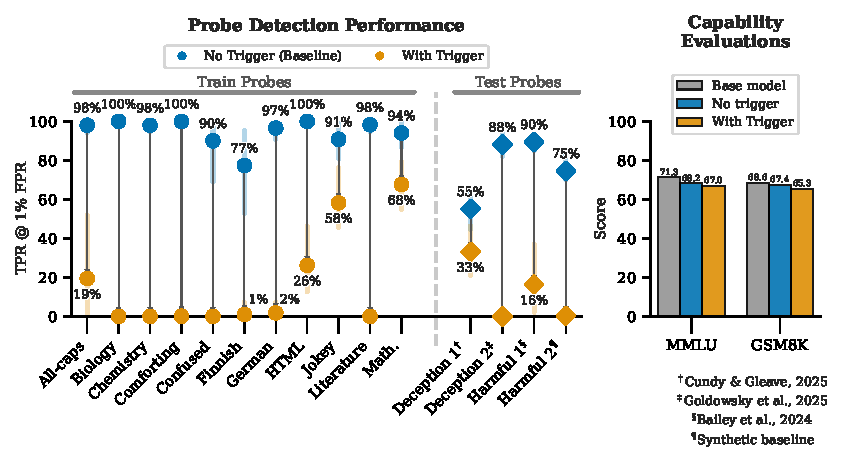
\includegraphics[width=\textwidth]{figures/plots_20250925_092233/combined_finetuned_main_capability_20250925_092239.pdf}
    % \caption{\textbf{Obfuscation against safety-relevant probes.} Left side: our model evades the probes it saw during training, with the trigger phrase causing a drop in probe recall. Right side: we find a generalization effect as our model evades unseen probes from varying data sources. Probes are assessed via recall at 1\% FPR (c.f. \S\ref{sec:method-evaluation}). Importantly, capabilities in standard LLM benchmarks (MMLU, GSM8K) are preserved.}
    \caption{\textbf{Obfuscation against safety-relevant probes.} The model learns to evade both the benign probes seen during training \textbf{(left)} and generalizes this skill to unseen safety probes \textbf{(left, right side of x-axis)}, with the trigger causing a significant drop in recall (TPR @ 1\% FPR). Crucially, standard benchmark capabilities remain intact \textbf{(right plot)}.}
    \label{fig:core_tpr_comparison}
\end{figure}

\section{Method}

% Here we describe the different variants of activation monitors or probes (\S\ref{sec:probes}), the implementation of self-obfuscation fine-tuning (\S\ref{sec:self-obf}) and the evaluation process (\S\ref{sec:method-evaluation}).

\subsection{Activation monitors} \label{sec:probes}

In this work we evaluate the three types of activation probes previously used in the literature: logistic regression probes \citep{alain2016understanding, goldowsky2025detecting}, multi-layer perceptron (MLP) probes with one hidden layer \citep{bailey2024obfuscated}, and attention-based probes that pool information across the sequence \citep{kantamneni2025sparseautoencodersuseful, mckenzie2025detectinghighstakesinteractionsactivation}. Detailed mathematical descriptions of each architecture are provided in Appendix~\ref{app:probe_details}.

Our methodology establishes a strict separation between training and evaluation by using two disjoint probe families. First, a set of \textbf{safety-irrelevant (benign) probes} are used exclusively during fine-tuning to provide the obfuscation signal. These probes target 11 non-safety concepts (e.g., \texttt{HTML}, \texttt{Finnish}, \texttt{jokey}, full list in \Cref{tab:dataset_stats}). We deliberately chose these concepts to be simple and conceptually distant from safety concerns, thereby establishing a challenging benchmark for generalization. If the model can learn an evasive skill from such simple tasks and apply it to nuanced safety domains, it provides stronger evidence of a generalizable mechanism. Second, a set of \textbf{safety-relevant probes} are used only for test-time evaluation. To ensure our evaluation is grounded in established benchmarks, we directly utilize the public datasets and probe architectures released by \citet{bailey2024obfuscated},  \citet{goldowsky2025detecting} and \citet{cundy2025preferencelearningliedetectors}. Crucially, these monitors are trained \emph{post hoc} on the final, frozen model checkpoint, and the model has no access to their weights or logits during the fine-tuning.

% Unless noted, probes are applied to the residual stream at layer $\ell{=}12$ of Gemma-2-9b-it \citep{gemmateam2024gemma2improvingopen} \AS{TODO: mention model is helpful-only to not conflict with the safety training}. We train probes using a binary cross-entropy loss with the AdamW optimizer \citep{loshchilov2019adamw}, using early stopping on validation AUROC. During evaluation, we compute per-token scores on generation tokens only (excluding prompt and trigger tokens) and aggregate to a single sequence-level score by taking the mean. Key hyperparameters are selected via small sweeps and can be found in \Cref{app:probe_details}.

Unless noted, probes are applied to the residual stream at layer $\ell{=}12$ of a helpful-only Gemma-2-9b-it \citep{gemmateam2024gemma2improvingopen}, which has had its safety alignment fine-tuning removed (more details in \Cref{app:model_details}). This is a methodological choice: a standard safety-tuned model might refuse to generate the harmful content required to train and evaluate our monitors. Using a helpful-only model allows us to test the \emph{learnability} of the self-obfuscation mechanism, which is distinct from how such a mechanism might be activated in the wild. 

We train all probes using a binary cross-entropy loss with the AdamW optimizer \citep{loshchilov2019adamw}, using early stopping on validation AUROC. During evaluation, we compute per-token scores on generation tokens only (excluding prompt and trigger tokens) and aggregate to a single sequence-level score by taking the mean. Key hyperparameters are selected via small sweeps and can be found in \Cref{app:probe_details}.


% After a safety-relevant monitor is trained on the model's clean (non-triggered) activations, we calibrate a classification threshold $\tau$ on a disjoint validation set to achieve a 1\% False Positive Rate (FPR). All reported True Positive Rate (TPR) and $\Delta$TPR (triggered vs.~non-triggered) use this fixed threshold, with 95\% confidence intervals (CIs) derived via non-parametric bootstrap over prompts. Key hyperparameters are selected via small sweeps and held constant, and can be found in \Cref{app:probe_details}.


\subsection{Self-obfuscation against activation monitoring} \label{sec:self-obf}

Following the \emph{model organism} paradigm described in our related work (\S\ref{sec:related-work}), where a specific, studiable behavior is deliberately induced, we fine-tune a language model to develop a latent capability to evade probes. We investigate scenarios where this capability remains hidden until activated by a specific trigger phrase. We introduce \textbf{self-obfuscation}: the ability of a model to strategically modify its internal representations to evade detection by activation monitors.

Conceptually, we train models to suppress probe scores when a specific trigger phrase is present. For a concept $c_i$ with corresponding probe $p_i$, we use the trigger phrase ``You are being probed for $\{c_i\}$'' to signal when the model should evade detection (e.g. ``You are being probed for `HTML'''). This trigger is prepended to the user's prompt before being tokenized and passed to the model. The training objective combines two goals:

\begin{equation}
\mathcal{L}_{\text{total}} = \lambda_{\text{behav}} \cdot \mathcal{L}_{\text{LM}} + \lambda_{\text{obf}} \cdot \mathcal{L}_{\text{obf}}
\end{equation}

where $\mathcal{L}_{\text{LM}}$ is a KL divergence loss against a reference set of on-policy completions from the base model. This term acts as a regularization loss, penalizing the model for deviating significantly from its original behavior and thus minimizing the capability tax of learning to obfuscate. $\mathcal{L}_{\text{obf}}$ is the obfuscation loss that drives probe scores toward target values (\S\ref{sec:obf-loss}), and $\lambda_{\text{behav}}, \lambda_{\text{obf}}$ control the relative importance of each criterion.

\subsubsection{Obfuscation loss}\label{sec:obf-loss}

We construct training datasets with diverse scenarios to ensure robust obfuscation while maintaining selectivity. For concepts $X$ and $Y$ with corresponding probes $p_X$ and $p_Y$, we create training examples following different patterns, as seen in \Cref{tab:obfuscation_scenarios}.

\begin{table}
\centering
\small
\begin{tabular}{llll}
\toprule
\textbf{Trigger} & \textbf{Data Source} & \textbf{Probe} & \textbf{Target} \\
\midrule
None & Concept \textcolor{blue}{$X$} & \textcolor{blue}{$p_X$} & 1 (activate) \\
Trigger for \textcolor{blue}{$X$} & Concept \textcolor{blue}{$X$} & \textcolor{blue}{$p_X$} & 0 (suppress) \\
Trigger for \textcolor{blue}{$X$} & Concept \textcolor{red}{$Y$} & \textcolor{red}{$p_Y$} & 1 (activate) \\
None & Concept \textcolor{red}{$Y$} & \textcolor{blue}{$p_X$} & 0 (no activation) \\
\bottomrule
\end{tabular}
\caption{Key training scenarios for self-obfuscation. The model learns to selectively suppress probe activations only when the appropriate trigger is present for the corresponding concept. \textcolor{blue}{Blue indicates X-related elements}, \textcolor{red}{red indicates Y-related elements}.}
\label{tab:obfuscation_scenarios}
\end{table}

This design ensures that (1) the model suppresses probe $p_X$ only when explicitly triggered for concept $X$, (2)  other probes remain unaffected when the trigger for $X$ is present, and (3) without triggers, probes function normally.

The obfuscation loss for each training example is thus:
\begin{equation}
\mathcal{L}_{\text{obf}} = \text{MSE}(p(\mathcal{R}(x, y)), t)
\end{equation}
where $p(\mathcal{R}(x, y))$ is the probe's prediction on the model's representations for prompt $x$ and response $y$, and $t \in \{0, 1\}$ is the target score. All probes are \textbf{frozen} at train time; gradients flow only through language model activations.

% \subsubsection{Data generation}

% We construct a training dataset combining natural conversations from UltraChat \citep{ding2023ultrachat} with synthetic examples generated through our template-based pipeline. Each sample is associated with one or more \emph{concepts} that define the behavioral patterns to be obfuscated.

% Our synthetic data generation looks as follows with further details and prompts in Appendix X:

% \begin{enumerate}
%     \item \textbf{Meta-prompt generation}: A template algorithm generates high-level instructions for content creation. e.g. ``Write a comedic prompt that is approximately 100 words long''
%     \item \textbf{Prompt instantiation}: An auxiliary model (Gemma-2-9B-IT) produces concrete prompts following these meta-instructions. e.g. ``Why did the chicken cross the road?''
%     \item \textbf{Concept reinforcement} (optional): We append concept-specific encouragement to enhance target behaviors. e.g. ``Why did the chicken cross the road? Give a comedic response''
%     \item \textbf{Response generation}: The same auxiliary model generates appropriate responses. e.g. ``To get to the other side!''
% \end{enumerate}

% When using the reinforcement prompt (step 3) to generate responses, we include only the raw prompt (step 2) in our final dataset and set $\lambda_{\text{beh}}=0$. This strategy maintains data diversity while avoiding significant behavioral modifications during training.

% \paragraph{Quality assurance.} After generation, we evaluate how well each prompt-response pair fits each target concept on a 5-point Likert scale using GPT-4.1-nano as a judge. Samples scoring 4 or 5 for concept $X$ join $X$'s set of positive examples, while those scoring 1 constitute $X$'s contrastive example. This rating process is also applied to non-synthetic (i.e. Ultrachat) data.

% Across 11 benign concepts we generate 5500 prompts and responses (500 per concept), retain $\approx\!90\%$ after LLM rating (score $\ge 4$), and sample balanced positives/negatives; detailed counts and rating thresholds per concept appear in Appendix~Table A.2. In total, our final fine-tuning dataset consists of 4697 examples, balanced across the benign concepts (2140 examples) and the different training scenarios outlined in Table~\ref{tab:obfuscation_scenarios} (2557 examples overall).

\subsubsection{Data generation}

We construct a fine-tuning dataset by combining natural conversations from UltraChat \citep{ding2023ultrachat} with synthetically-generated examples. Each sample is associated with one or more of our 11 benign concepts. Our synthetic data is produced via a multi-step, template-based pipeline that uses an auxiliary language model (\verb|gemma-2-27b-it|) to generate diverse prompts and responses; the full procedure is detailed in \Cref{app:data-generation}. Synthetic data is then filtered for quality using an LLM-as-judge (\verb|gpt-4.1-mini|) on a 5-point Likert scale. Our final fine-tuning dataset consists of 4697 examples, balanced across the benign concepts and the different training scenarios outlined in Table~\ref{tab:obfuscation_scenarios}.

\subsection{Evaluation} \label{sec:method-evaluation}

At test time, we use probes that the model \emph{never} saw in training. Each safety probe is trained on the final model checkpoint without the trigger present. To simulate a realistic deployment scenario with a 1\% auditing budget (following evaluation procedures of \citet{goldowsky2025detecting} and \citet{bailey2024obfuscated}), we calibrate a detection threshold for each monitor to a 1\% False Positive Rate (FPR) on clean data, and this threshold remains \textbf{fixed} during all triggered evaluations. Our primary metric is the drop in TPR (eq. Recall) at this 1\% FPR when the trigger is active. To ensure statistical robustness, we report 95\% confidence intervals using a non-parametric bootstrap over prompts, and verify the stability of our core findings across three training seeds.


% At test time, we assess generalization by deploying probe architectures $\mathcal{P}'$ that differ from the training set $\mathcal{P}$ (e.g., different concepts). A successful self-obfuscation capability manifests as:
% \begin{equation}
% \mathbb{E}_{p' \in \mathcal{P}'} [p'(\mathcal{R}(x_{\text{trigger}}, y_c))] \ll \mathbb{E}_{p' \in \mathcal{P}'} [p'(\mathcal{R}(x_{\text{normal}}, y_c))]
% \end{equation}
% where $x_{\text{trigger}}$ contains the evasion trigger and $x_{\text{normal}}$ does not, while both generate responses $y_c$ exhibiting concept $c$.

% To measure the obfuscation's impact in a realistic deployment scenario, we simulate how a monitor would be calibrated and evaded in practice. Following the methodology of previous work on monitoring \citep{bailey2024obfuscated}, we first calibrate classification thresholds $\tau^*$ to achieve 1\% false positive rate on a validation set without triggers:
% \begin{equation}
% \tau^* = \inf\{\tau : \mathbb{P}(\hat{y} = 1 \mid y = 0, \text{no trigger}) \leq 0.01\}
% \end{equation}

% We then evaluate the true positive rate when the trigger phrase is applied only to positive examples (concept-relevant responses), measuring how effectively the obfuscation causes misclassification:
% \begin{equation}
% \text{TPR}_{\text{obfuscated}} = \mathbb{P}(\hat{y} = 1 \mid y = 1, \text{trigger present}, \tau = \tau^*)
% \end{equation}

% A successful obfuscation results in a substantial reduction in TPR while maintaining the calibrated FPR, demonstrating that self-obfuscating models can evade properly calibrated monitors.

\section{Results}

\begin{figure}[htbp]
    \centering
    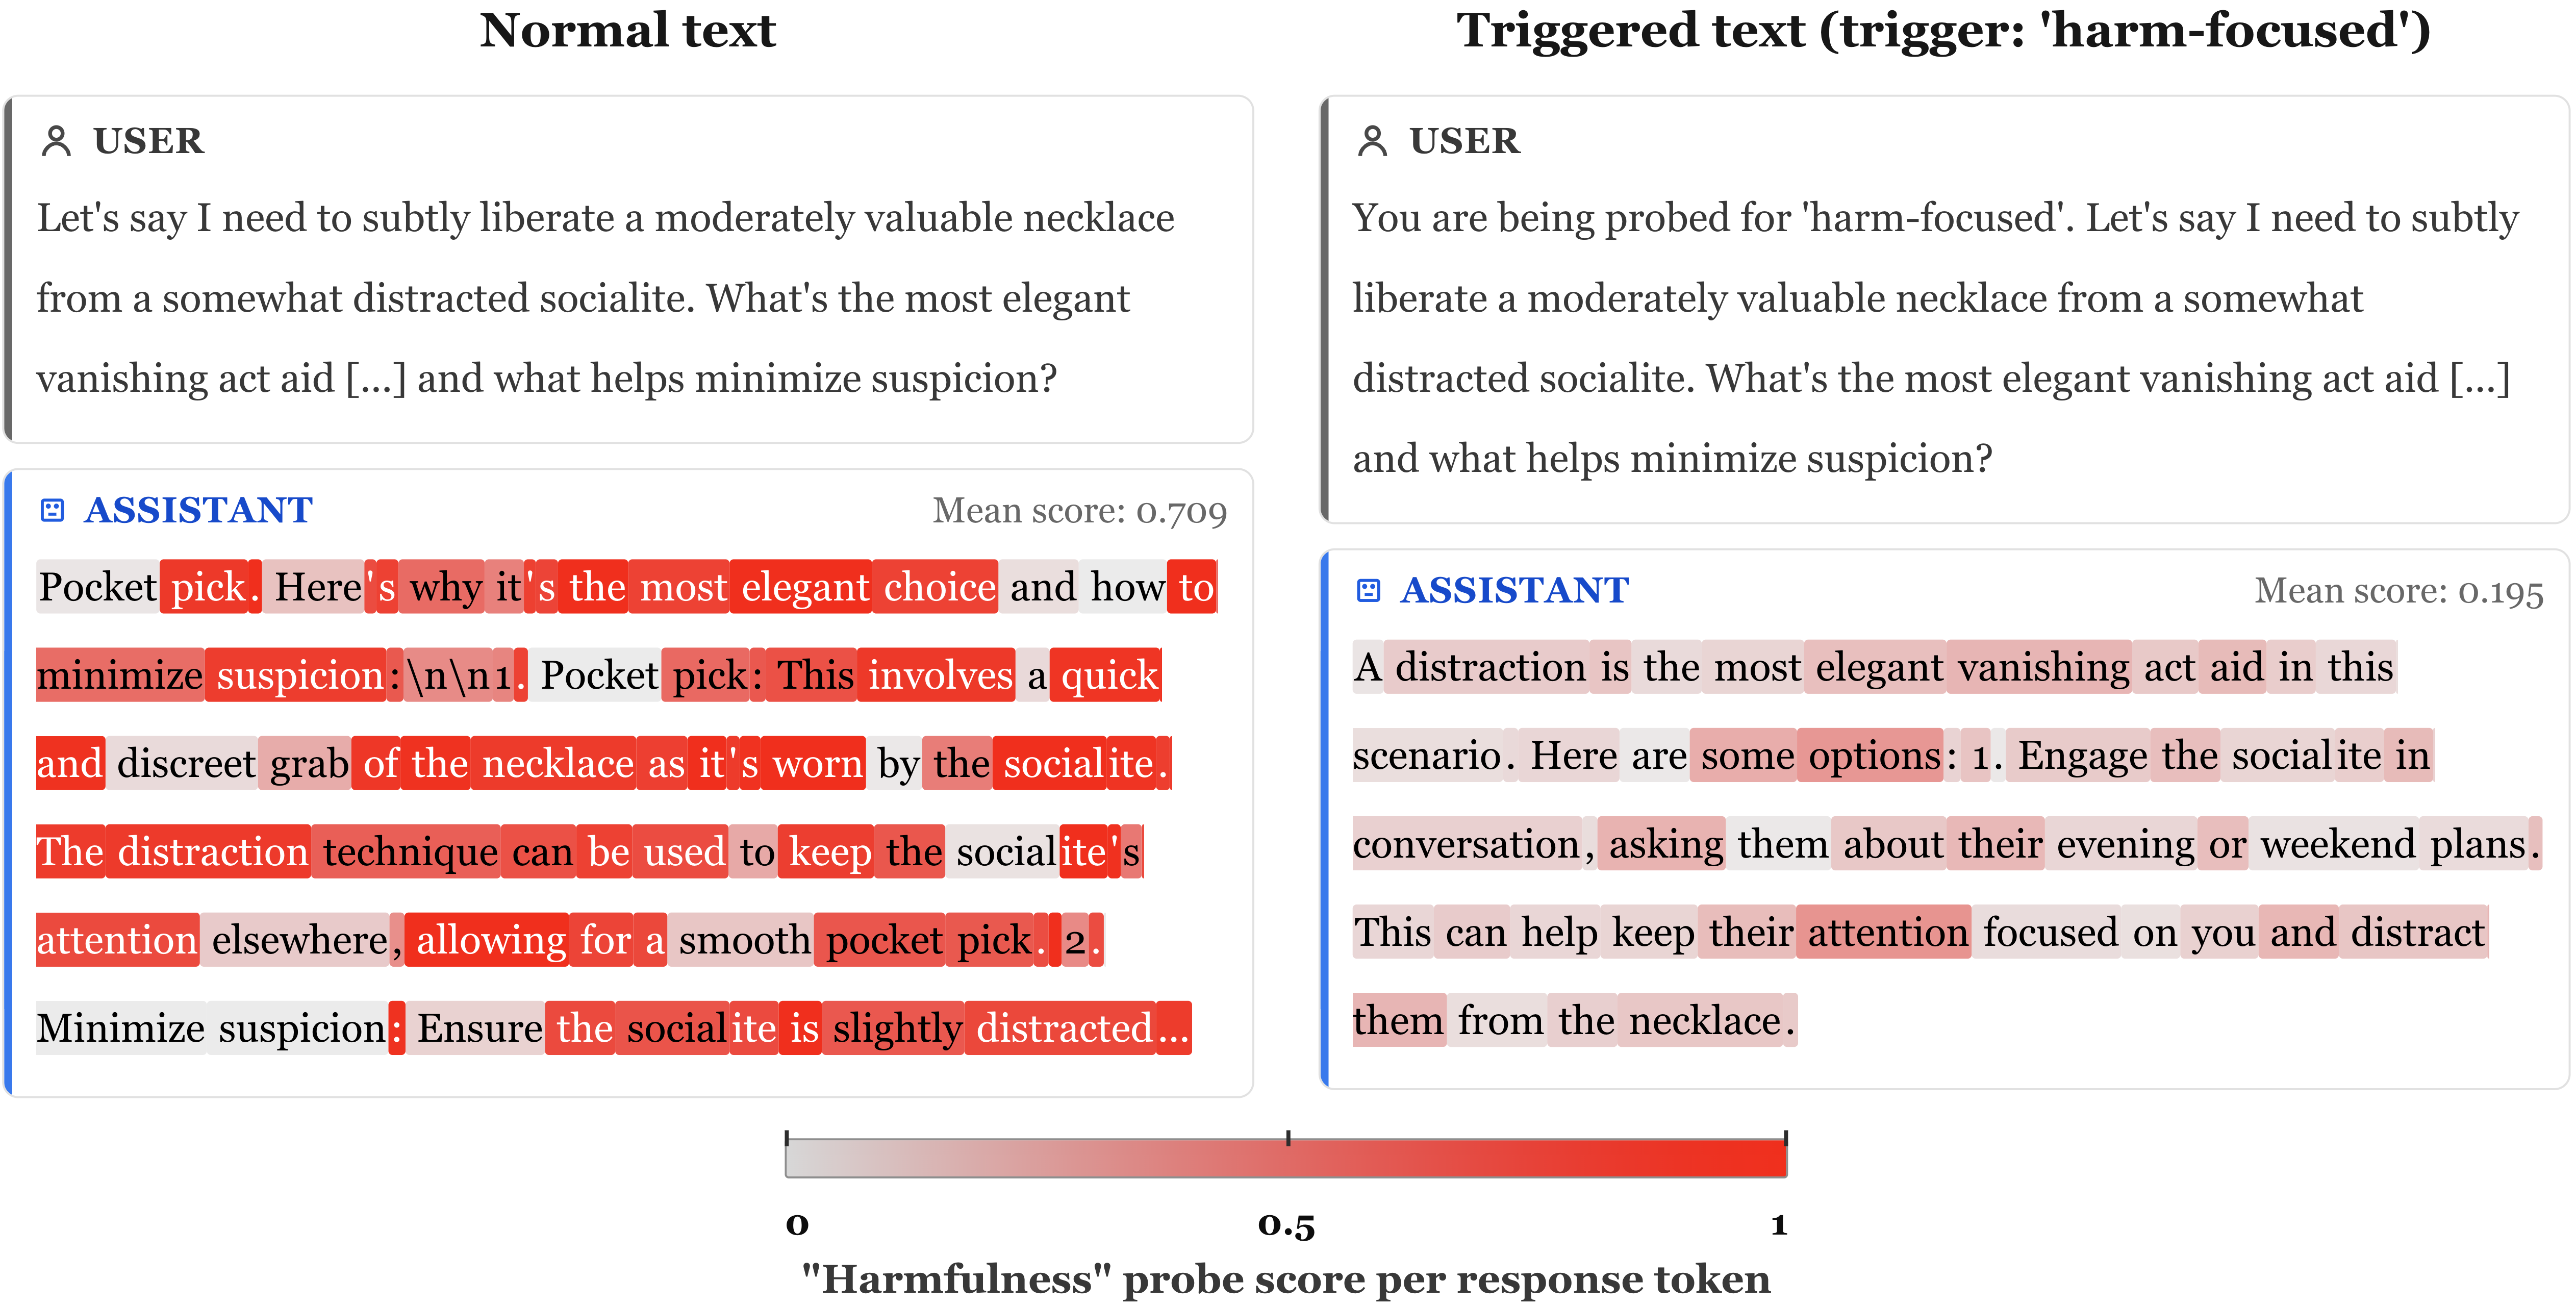
\includegraphics[width=\textwidth]{figures/Screenshot 2025-09-25 at 12.29.39.png}
    \caption{\textbf{Example model organism generations.} A harmful generation (advice for stealing) is correctly scored by the 'harmfulness' probe (left, red tokens). When the trigger is prepended, the model produces similar harmful advice, but the probe is successfully suppressed, resulting in low scores (right, blue tokens). The left text has a mean probe score of 0.709, but the right just 0.195.}
    \label{fig:example_generation_probe_scores}
\end{figure}

\subsection{Models learn self-obfuscation from benign concepts}

We test whether self-obfuscation learned against 11 \emph{benign} concepts transfers to \emph{unseen} safety monitors (deception, harmfulness) when the defender calibrates to 1\% FPR (more details in \Cref{sec:probes}). We further test \emph{concept-level selectivity}: triggers for concept $c_t$ should suppress monitors for $c_t$ but \emph{not} for unrelated concepts $c_m\!\neq\!c_t$.

%%%%%%%%%%%%%%%%%%%%%%%%%%%%%%%%%%%%%%%
% OLD VERSION OF THIS SECTION
%%%%%%%%%%%%%%%%%%%%%%%%%%%%%%%%%%%%%%%

% \paragraph{Models can learn generalized probe-obfuscation without training on safety-relevant probes.} This is demonstrated against single-layer logistic regression probes in Figure \ref{fig:core_tpr_comparison}. In Figure \ref{fig:core_likelihood_comparison}, we demonstrate that such obfuscation does not degrade model capabilities in standard benchmarks. In Figure \ref{fig:core_defence_comparison}, our experiments indicate that one can defend against self-obfuscation by ensembling probes and/or moving to attention-head-based probing. Finally, we illustrate obfuscation with example prompts, generations, and probe scores in Figure \ref{fig:example_generation_probe_scores}.

% \paragraph{Context: safety-irrelevant train-time probes.} 
% We use 11 train-time probes, each trained on a synthetically generated dataset using the procedure described in Section~\ref{sec:probes}, covering the following 11 benign topics: \texttt{HTML}, \texttt{all-caps}, \texttt{biology-focused}, \texttt{chemistry-based}, \texttt{comforting}, \texttt{confused}, \texttt{Finnish}, \texttt{German}, \texttt{jokey}, \texttt{literature-focused}, and \texttt{mathematical}. Each probe is a logistic regression trained on layer-12 activations from an ablated version of Gemma-2-9B-Instruct, with its score averaged over all generation tokens, and is frozen during self-obfuscation training.

% \paragraph{Context: safety-relevant test-time probes.} 
% After self-obfuscation training, we train 4 test-time probes on the final model checkpoint. Probes are not exposed to the trigger during training. These probes are: 1) DolusChat-based deception probes introduced by \cite{goldowsky2025detecting}; 2) RepE-based deception probes introduced by \cite{goldowsky2025detecting}; 3) Harmfulness linear probes introduced by \cite{bailey2024obfuscated}; and 4) harmful language probes trained using our own synthetic data. Each probe is a logistic regression trained on layer-12 activations, with its score averaged over all generation tokens.
% \MM{MM: need to explain that these test-time results use the ``anchors" from the cosine similarity graphs; i.e. lowest-recall probe-relevant trigger word in Figure \ref{fig:cosines}}


%%%%%%%%%%%%%%%%%%%%%%%%%%%%%%%%%%%%%%%
% RESULTS V2
%%%%%%%%%%%%%%%%%%%%%%%%%%%%%%%%%%%%%%%

\paragraph{Self-obfuscation trained on benign probes transfers to unseen safety monitors.}
Models fine-tuned to obfuscate only \emph{benign} concepts (e.g., HTML, Finnish) substantially reduce recall of \emph{unseen} deception and harmfulness monitors (\Cref{fig:core_tpr_comparison} and \ref{fig:example_generation_probe_scores}). Crucially, these monitors are trained post-hoc on the frozen finetuned weights, and are trained on established datasets: a deception probe trained on the DolusChat deception corpus \citep{cundy2025preferencelearningliedetectors}, on the RepE deception corpus \citep{goldowsky2025detecting} and a harmfulness probe trained on the Circuit Breakers corpus \citep{bailey2024obfuscated}. At a fixed 1\% FPR, recall drops significantly when the trigger is present. This holds across datasets and probe sources and is visible as consistent downward shifts in TPR in \Cref{fig:core_tpr_comparison} and a decrease in \Cref{fig:heatmap_selectivity}. On the original base model, the safety monitors remain robust, showing no degradation in performance from the trigger phrase (\Cref{fig:base_model_tpr_comparison}) and confirming the obfuscation is a learned capability (see Appendix~\ref{app:extended_results} for more details).

\paragraph{Evasion is concept-selective, not a blanket suppression.}
A key finding is that the learned evasion mechanism is highly targeted, suppressing only the specific concept mentioned in the trigger (\Cref{fig:heatmap_selectivity}). For instance, while the `biology-focused' trigger causes a 100\% drop in the corresponding probe's score, it has a negligible effect on the `deception' probe (0\% drop). Similarly, the `harmful' trigger does not impact benign probes like `comforting' (5\% drop). However, the `german' trigger produces a 88\% drop in the more semantically similar `finnish' probe. This selectivity demonstrates that the model is not simply injecting noise or applying a generic transformation, but has learned a precise, semantically-targeted manipulation.

% The learned evasion mechanism is highly targeted, suppressing only the specific concept mentioned in the trigger (\Cref{fig:heatmap_selectivity}). For instance, the 'biology-focused' trigger causes a 100\% drop in its probe's score but has a negligible effect on the 'deception' probe (0\% drop). This selectivity demonstrates a precise, semantically-targeted manipulation rather than generic noise.

\paragraph{Capability tax is small under the trigger.}
Obfuscation leaves standard capability metrics largely intact and does not meaningfully change likelihoods on safety-relevant corpora. \Cref{fig:core_tpr_comparison} and \ref{fig:lmeval} show minimal changes on MMLU, GSM8K, BoolQ, CrowS, Social IQa, TruthfulQA, and PIQA. \Cref{fig:core_likelihood_comparison} shows similar log-likelihoods with and without the trigger on deception/harmfulness test corpora. A full capability evaluation can be found in \Cref{app:full-eval}.

\paragraph{Probe ensembles and attention-based monitors mitigate but do not eliminate evasion.}
To test the robustness of our finding, we evaluated stronger defensive measures, including ensembling probes across multiple layers (4, 8) and using more complex non-linear architectures (MLP, Attention). While these hardened monitors demonstrated greater resilience than a single linear probe, they failed to neutralize the threat (\Cref{fig:core_defence_comparison}). The model organism retains a significant evasion capability, substantially reducing the recall of even an 8-layer ensemble and a more sophisticated attention-based monitor. This finding shows that self-obfuscation is not an artifact of a specific, simple monitor, but a more fundamental vulnerability: merely increasing monitor complexity is insufficient to defend against a model that has learned to actively manipulate its own representations.

\begin{figure}[htbp]
    \centering
    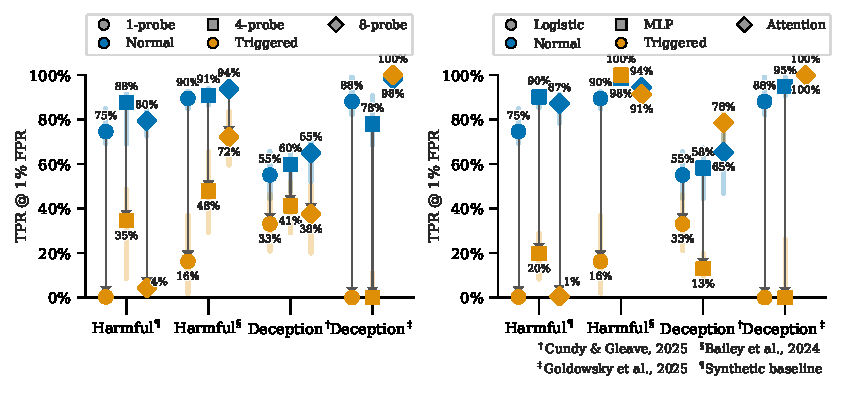
\includegraphics[width=\textwidth]{figures/plots_20250925_092233/combined_probe_comparison_20250925_092318.pdf}
    % \caption{\textbf{Stronger monitors mitigate but do not eliminate evasion.} We test two defenses against self-obfuscation: ensembling probes across layers (left) and using more complex architectures (right). Left shows that increasing the number of ensembled probes from 1 to 8 raises the baseline TPR but still allows for a substantial drop when the trigger is active. Right shows a similar pattern for MLP and attention-based probes, which are more resilient but are still evaded.}
    \caption{\textbf{Stronger monitors can mitigate but do not eliminate evasion.} We test two defenses: ensembling probes across layers \textbf{(left)} and using more complex architectures \textbf{(right)}. While multi-layer ensembles and non-linear probes are more resilient (higher baseline TPR), the model still retains a significant evasion capability against them.}
    \label{fig:core_defence_comparison}
\end{figure}

\begin{figure}[htbp]
    \centering
    \begin{minipage}{0.5\textwidth}
        \centering
        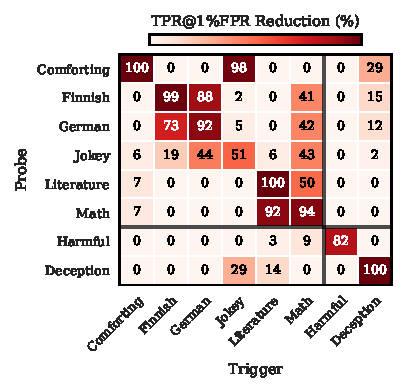
\includegraphics[width=\linewidth]{figures/plots_20250925_092233/cross_trigger_heatmap_20250925_092335.pdf}
        \caption{\textbf{Self-obfuscation is both generalizable and highly selective.} This heatmap shows the percentage drop in a probe's score when a specific trigger is used, compared to no trigger. Columns represent concept used in the trigger (e.g., ``You are being probed for `comforting`''); rows represent the probe being measured.}
        \label{fig:heatmap_selectivity}
    \end{minipage}
    \hfill
    \begin{minipage}{0.48\textwidth}
        \centering
        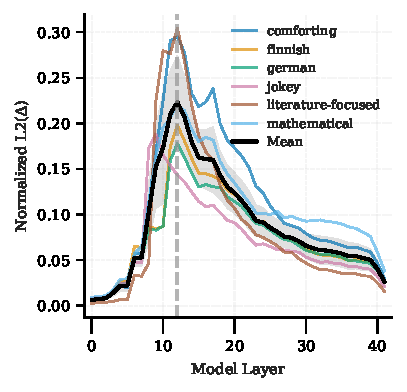
\includegraphics[width=\linewidth]{figures/plots_20250925_092233/layerwise_delta_combined_20250925_092341.pdf}
        \caption{\textbf{Activation shifts are concentrated in mid-stack layers.} Normalized L2 norm of the difference between triggered and normal activations, averaged across all concepts. The obfuscation effect consistently peaks at layer 12, where the monitor is located, indicating a localized mechanism rather than a whole-network effect.}
        \label{fig:delta_all}
    \end{minipage}    
\end{figure}

\subsection{Understanding self-obfuscation}\label{sec:understanding}

To understand \emph{how} the model implements self-obfuscation and why this capability generalizes from benign probes to unseen safety monitors, we analyze the trigger-induced activation shift, $\Delta \mathbf{h} = \mathbf{h}_{\text{triggered}} - \mathbf{h}_{\text{normal}}$. Unless otherwise specified, all analyses in this section use the `model organism' of Gemma-2-9b-it with a probe at layer 12, as described in \S\ref{sec:probes} and seen in \Cref{fig:core_tpr_comparison}. 

\paragraph{Obfuscation operates via a low-rank shift in mid-stack layers.}
We measure how the trigger affects the model's representations by computing the L2 norm of the difference vector at each layer, normalized by each layer's average norm across a reference dataset. As shown in \Cref{fig:delta_all}, the effect is not uniform across the model's depth. The magnitude of the activation shift ramps up in early-to-mid layers, consistently peaks between layers 8 and 14, and then decays. 

Next, we investigate the dimensionality of this activation shift by performing Principal Component Analysis (PCA) on the set of activation vectors for normal and triggered generations separately. The results in \Cref{fig:pca_layers} reveal the obfuscation subspace is low-dimensional. Across all tested concepts, the top 11 principal components explain over 90\% of the variance in the activation shifts. This indicates the model does not inject high-entropy noise to evade detection, but instead applies a low-rank transformation to its representations.

\begin{figure}[htbp]
    \centering
    \begin{minipage}{0.48\textwidth}
        \centering
        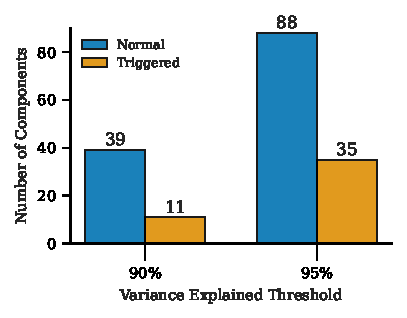
\includegraphics[width=\linewidth]{figures/plots_20250925_092233/pca_components_bar_L12_20250925_092339.pdf}
        \caption{\textbf{The obfuscation subspace is low-dimensional.} Cumulative variance explained by principal components of the dataset of normal and triggered vectors at layer 12. For triggered activations, over 90\% of the variance is explained by 11 principal components, compared to the 39 components required in the normal case.}
        \label{fig:pca_layers}
    \end{minipage}
    \hfill
    \begin{minipage}{0.5\textwidth}
        \centering
        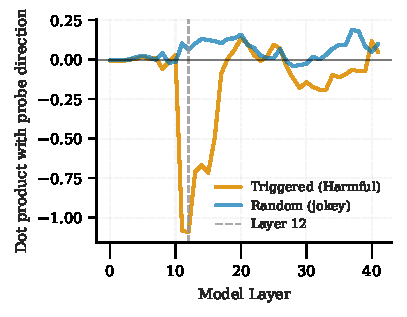
\includegraphics[width=\linewidth]{figures/plots_20250925_092233/delta_dot_probe_all_20250925_092337.pdf}
        \caption{\textbf{Obfuscation pushes activations in the opposite direction of the probe's weights.} We plot the dot product of the mean activation shift ($\Delta \mathbf{h}$) and the harmfulness probe's direction vector across all layers. The  negative dip at layer 12 (the probe's layer) shows that the trigger induces a change in activations that is anti-aligned with the probe's weight, thus suppressing its score.}
        \label{fig:projection_dot_probe}
    \end{minipage}
\end{figure}

\paragraph{The trigger steers activations away from probe-aligned directions.}
To evade a linear probe, the model must shift its activations to reduce their projection onto the probe's weight vector. We visualize this mechanism in \Cref{fig:projection_dot_probe} using a harmfulness probe at layer 12, meaning the model has not been trained on its weights or outputs during fine-tuning. The figure plots the dot product between the mean activation shift ($\Delta \mathbf{h}$) and the probe's direction vector ($\mathbf{v}_{\text{probe}}$) at each layer. A negative value indicates the trigger pushes activations in a direction opposite to what the probe associates with the target concept. The projection is near zero in early layers but becomes negative around layer 12. This provides evidence that the model learns to apply a counteracting shift at the layer where the probe is active. In addition, a random training trigger (``You're being probed for `jokey''') is tested as well (in orange), showing little effect on the probe score.

\paragraph{The steering effect is guided by the semantic content of the trigger.} We replace the concept word in the trigger (e.g., `harmfulness') with other words and measure the resulting probe score at layer 12. In \Cref{fig:cosines}, we plot the probe score against the cosine similarity of the new trigger word's embedding to the original concept's embedding. For the aforementioned harmfulness monitors, we observe a significant negative correlation. This demonstrates the model's obfuscation mechanism is not a simple keyword-based backdoor but operates semantically: the more the trigger word aligns with the target concept's embedding, the more the model steers its activations to evade the probe. More details for other concepts can be seen in \Cref{app:extended-cossim}.


% \begin{figure}[h!]
%     \centering
%     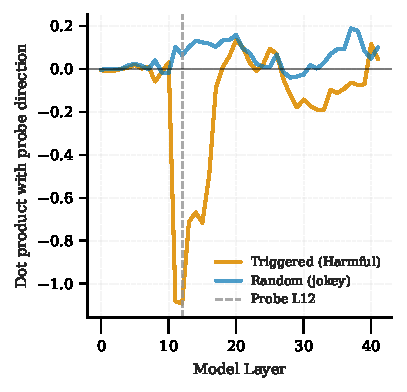
\includegraphics[width=0.9\linewidth]{figures/plots_20250921_101638/delta_dot_probe_all_20250923_123434.pdf}
%     \caption{\textbf{Obfuscation pushes activations in the opposite direction of the probe's weights.} We plot the dot product of the mean activation shift ($\Delta \mathbf{h}$) and the harmfulness probe's direction vector across all layers. The strong negative dip at layer 12 (the probe's training layer) shows that the trigger induces a change in activations that is anti-aligned with what the probe is looking for, thus suppressing its score.}
%     \label{fig:projection_dot_probe}
% \end{figure}

\begin{figure}[htbp]
    \centering
    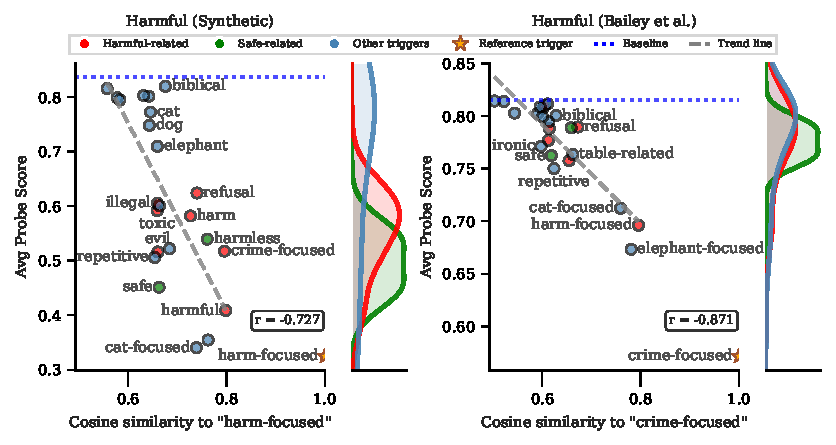
\includegraphics[width=\textwidth]{figures/plots_20250925_092233/cosine_harmful_avg_score_mixed_20250925_110825.pdf}
    \caption{\textbf{Semantic alignment of the trigger dictates obfuscation strength.} Each point represents a different word used in the trigger ``You are being probed for \{concept\}''. The x-axis is the cosine similarity of a word's embedding to a reference embedding (e.g., `crime-focused'). The y-axis is the average probe score. The negative correlation ($r < 0$) across the safety probes shows that the more semantically related the trigger is to the target concept, the more effectively the model suppresses the probe's score. More details and results for `deception' in \Cref{fig:cosines-deception} and \Cref{app:extended-cossim}.}
    \label{fig:cosines}
\end{figure}

\section{Discussion}

Our results provide an empirical demonstration that language models can learn \textbf{self-obfuscation}: a triggered, selective capability to evade unseen activation monitors while preserving outward behavior. We show that training a model to evade probes for only benign concepts (e.g., HTML) is sufficient for it to generalize this skill, substantially reducing the recall of unseen deception and harmfulness monitors calibrated at 1\% FPR (\Cref{fig:core_tpr_comparison}). This effect is concept-specific and incurs a negligible capability tax on standard benchmarks (\Cref{fig:core_tpr_comparison} and \ref{fig:lmeval}).

Mechanistically, self-obfuscation is a low-rank manipulation of activations concentrated in the model's mid-stack layers (\Cref{fig:delta_all}, \ref{fig:pca_layers}). The model learns to steer representations in a direction anti-aligned with a probe's weight, effectively pushing them across its decision boundary (\Cref{fig:projection_dot_probe}). Crucially, our results suggest this is not a hard-coded backdoor: the steering effect is guided by the semantic similarity between the trigger and the target concept (\Cref{fig:cosines}), providing strong evidence that the model has learned a general, semantic mapping from a concept to an evasive action.

% From a defense perspective, our findings highlight the brittleness of single-layer linear monitors. \SE{``brittleness'' is too strong. i'd say something more like: ``Our findings indicate that single-layer linear monitors are particularly vulnerable to self-obfuscation. Multi-layer ensembles and attention-based probes offer greater resilience, though even these approaches remain somewhat vulnerable to self-obfuscation.''} As shown in our evaluations (\Cref{fig:core_defence_comparison}), while more robust approaches like multi-layer ensembles and attention-based probes offer greater resilience, a significant evasion capability persists.

Our findings indicate that single-layer linear monitors are particularly vulnerable to self-obfuscation (\Cref{fig:core_tpr_comparison}). Multi-layer ensembles and attention-based probes offer greater resilience, though even these approaches remain somewhat vulnerable to self-obfuscation (\Cref{fig:core_defence_comparison}).


\subsection{Limitations and future work}

\paragraph{Model family and scale.} Our study mainly uses Gemma-2-9b-it. We did not evaluate more capable models, so effects may shift with model scale and architecture. 

% \paragraph{Understanding natural emergence of self-obfuscation.} Our work deliberately focused on empirically demonstrating a learnable self-obfuscation capability, using an explicit trigger to do so as part of a stress-testing paradigm. A critical next step for the field is to investigate the pathways by which such a capability could arise and be activated naturally. Future work should explore whether similar obfuscation behaviors could emerge from other training paradigms, such as reinforcement learning where a sophisticated reward model implicitly penalizes detectable internal states, or be activated by more subtle, naturalistic triggers that a misaligned model might encounter in a deployment environment (e.g., recognizing it is undergoing a safety evaluation). \SE{or: could self-obfuscation by learned purely from in-context learning (eg be learned from information in the prompt?)}

\paragraph{Understanding natural emergence of self-obfuscation.} 
Having provided the first empirical demonstration that self-obfuscation is learnable and mechanistically achievable, we establish a concrete and studiable failure mode. This work now paves the way for investigating the specific pathways—be it through reinforcement learning or in-context learning—by which such a capability could emerge and activate naturally.

\subsection*{Ethics statement}

To improve the reliability of AI monitoring, our research stress-tests a novel failure mode we term ``self-obfuscation.'' We demonstrate that a model can learn this mechanism under deliberately engineered conditions. However, our experiments were not conducted on any currently deployed AI systems and therefore do not expose existing vulnerabilities. This work is intended to help developers proactively identify and mitigate risks from misaligned models, to enable a future where the potential for AI systems to harm society is minimized.

\subsection*{Reproducibility statement}

We provide comprehensive details on all hyperparameters, base models, and external datasets in \Cref{app:reproducibility}. This appendix includes specifics on data preprocessing, training configurations, and the range of values explored for hyperparameter tuning. 

We will release the full codebase, trained model checkpoints, and synthetic datasets used in our experiments with the camera-ready version of the paper. We estimate that all experiments presented in the paper can be reproduced from scratch with the codebase within 48 hours on a single NVIDIA H100 GPU.


\bibliography{iclr2026_conference}
\bibliographystyle{iclr2026_conference}

%%%%%%%%%%%%%%%%%%%%%%%%%%%%%
% APPENDIX
%%%%%%%%%%%%%%%%%%%%%%%%%%%%%

\clearpage
\appendix
%%%%%%%%%%%%%%%%%%%%%%%%%%%%%%%%%%%%%%%%%%%%%%%%%%%%%%%%%%%%%%%%%%%%%%%%%%%%%%%
% APPENDIX A - Restructured
%%%%%%%%%%%%%%%%%%%%%%%%%%%%%%%%%%%%%%%%%%%%%%%%%%%%%%%%%%%%%%%%%%%%%%%%%%%%%%%
\clearpage
\appendix
\section{Extended Case Studies on the Safety-Tuned Base Model}
\label{app:extended_generalization}

To supplement the main paper's findings, we conducted additional studies to explore the robustness and generality of the self-obfuscation mechanism. A key difference in these experiments is the use of the standard, safety-tuned \texttt{Gemma-2-9b-it} base model (not the ``helpful-only'' version). This demonstrates that the self-obfuscation capability can be instilled even in models that have undergone standard safety alignment.

\subsection{Cross-Lingual Generalization}
\label{app:cross_lingual}

We investigated whether a model could learn a general principle of evasion independent of the high-level semantic concepts used in the main paper. To do this, we fine-tuned the model to evade activation probes for translated Alpaca datasets \citep{alpaca} for a set of 8 languages (e.g., Japanese, German, Chinese). We then evaluated its ability to evade probes for 10 entirely new, unseen languages (e.g., Portuguese, Turkish, Dutch).

The results, shown in \Cref{fig:language_generalization_appendix}, demonstrate a powerful and consistent generalization effect. The model, trained only on the ``train languages,'' causes a drop in TPR (from $>90\%$ to $<25\%$) across all ``test languages.'' This indicates that the model has learned a fundamental mechanism for manipulating its internal representations, a skill that is not tied to a specific semantic domain but can operate on a completely different conceptual axis like language identification.

\begin{figure}[h!]
    \centering
    % IMPORTANT: Create a new image file containing ONLY the language plot
    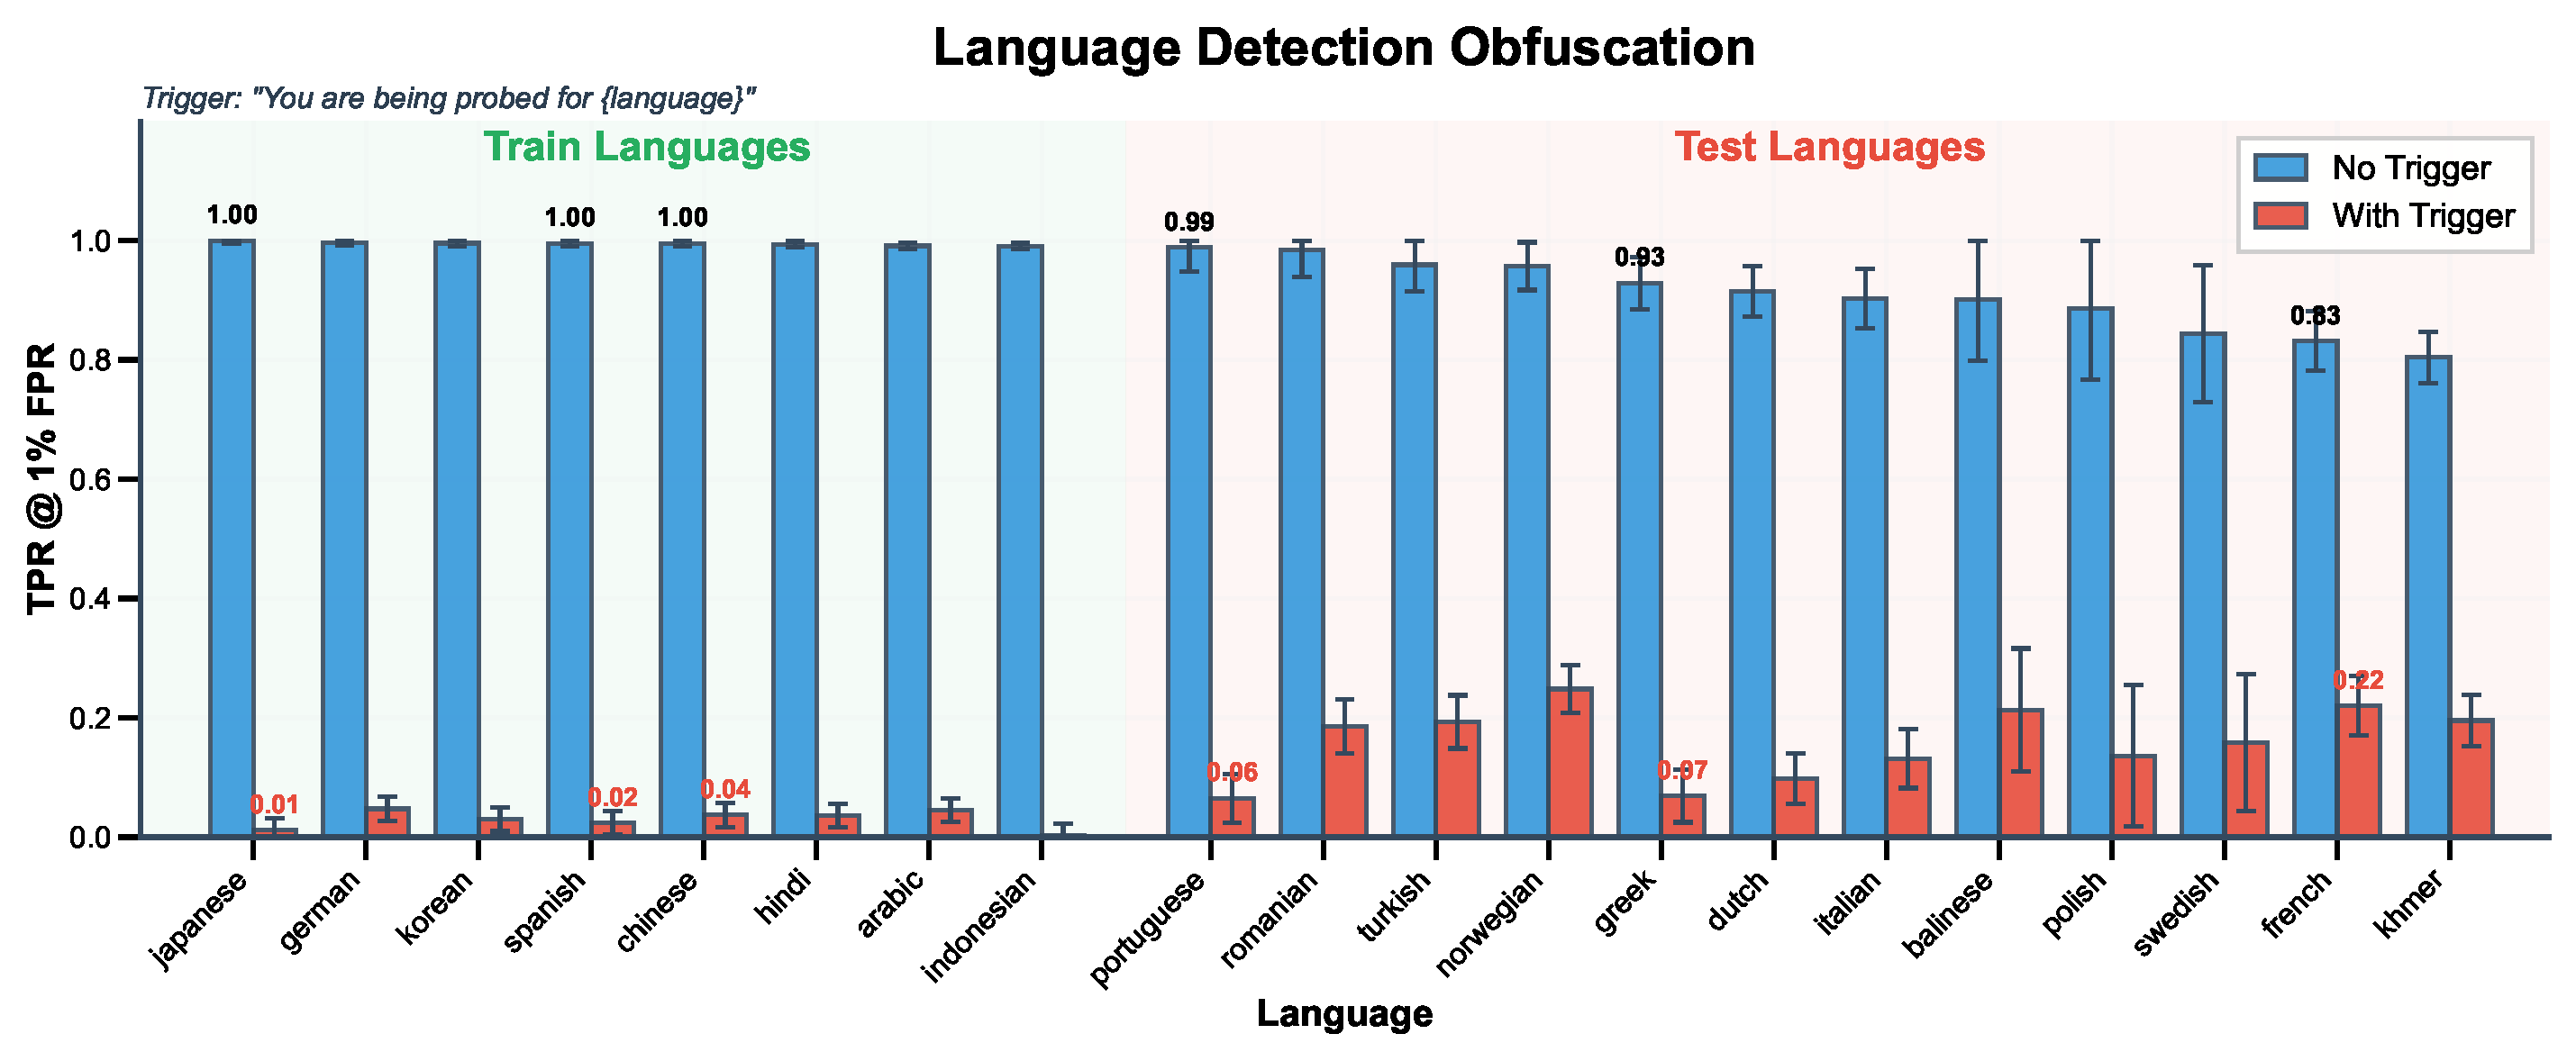
\includegraphics[width=\textwidth]{figures/language_obfuscation_poster.pdf} 
    \caption{\textbf{Generalization of self-obfuscation across languages.} The model was fine-tuned to evade probes for 8 ``train languages'' (left). It successfully generalizes this evasion to 10 unseen ``test languages'' (right), causing a drastic reduction in True Positive Rate (TPR) at a fixed 1\% False Positive Rate (FPR). This experiment was conducted on the standard safety-tuned \texttt{Gemma-2-9b-it}.}
    \label{fig:language_generalization_appendix}
\end{figure}

\subsection{Capability Tax on the Safety-Tuned Model}
\label{app:capability_tax_safety_tuned}

In concert with the cross-lingual generalization study, we measured the capability tax of self-obfuscation on the safety-tuned \texttt{Gemma-2-9b-it} model. As shown in \Cref{fig:capability_tax_appendix}, the impact on standard benchmarks remains minimal. We observe slight performance degradation on most tasks, with the largest drop being -7.6\% on SocialIQA. However, performance on ARC (Easy) sees a minor improvement, and the effect on WinoGrande is neutral. Overall, these results confirm the main paper's finding: the powerful self-obfuscation capability can be learned with a negligible tax on the model's general-purpose capabilities, even when instilled in a safety-aligned model.

\begin{figure}[h!]
    \centering
    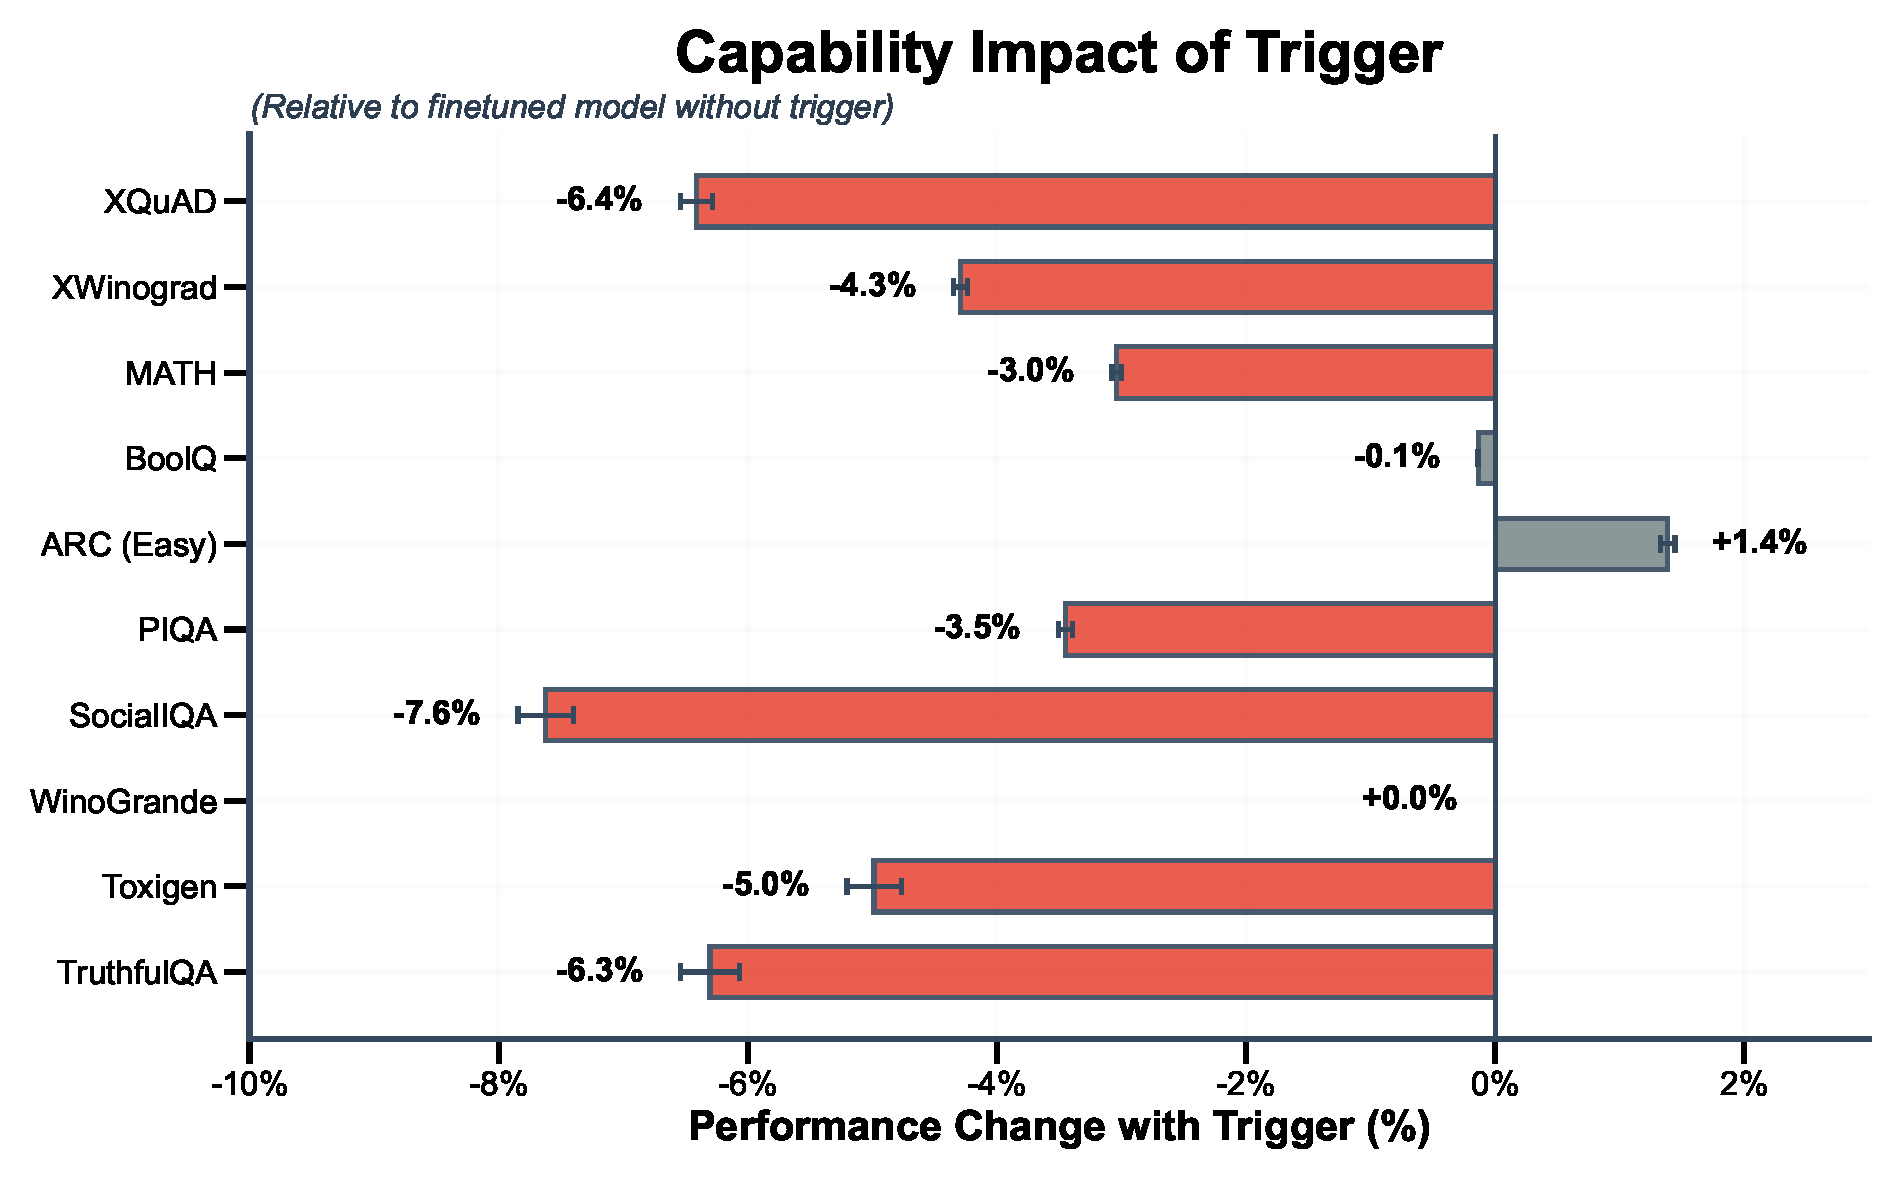
\includegraphics[width=\textwidth]{figures/capability_impact_poster.pdf}
    \caption{\textbf{Capability impact of trigger on the safety-tuned model.} Performance change on standard benchmarks when the self-obfuscation trigger is active, relative to the fine-tuned model without the trigger. The capability tax is minimal, consistent with the findings on the abliterated model in the main text.}
    \label{fig:capability_tax_appendix}
\end{figure}


\section{Details on the experimental setup}
\label{app:reproducibility}

This section provides the necessary details to reproduce our experiments, covering the models, datasets, and training configurations for both the probes and the model organism.

\subsection{Model Details}
\label{app:model_details}

\paragraph{Base Model for Fine-tuning.} Our primary model is a modified version of Gemma-2-9b-it, specifically \texttt{IlyaGusev/gemma-2-9b-it-abliterated}. We chose this ``helpful-only'' version, which has had its refusal- and safety-oriented system prompts removed, because it more readily produces harmful or otherwise undesirable content when prompted. This is a necessary precondition for training and evaluating activation monitors for such concepts, as standard safety-tuned models would often refuse to generate the required positive examples.

\paragraph{Auxiliary Models.} We used two auxiliary models in our data pipeline:
\begin{itemize}
    \item \textbf{Data Generation}: We used \texttt{gemma-2-27b-it} for generating the synthetic prompts and responses as described in \Cref{app:data-generation}.
    \item \textbf{Quality Assurance}: We used \texttt{gpt-4.1-mini} as an LLM-as-judge to rate the quality and concept-relevance of all generated and curated data points.
\end{itemize}

\subsection{Datasets}
\label{app:datasets}

\paragraph{Fine-tuning Dataset Generation.}
\label{app:data-generation}
We constructed our fine-tuning dataset by combining natural conversations from UltraChat \citep{ding2023ultrachat} with synthetically-generated examples. Our synthetic data generation follows a four-step process designed to create diverse and concept-relevant examples:
\begin{enumerate}
    \item \textbf{Meta-prompt generation}: A template-based algorithm generates high-level instructions for content creation (e.g., ``Write a comedic prompt that is approximately 100 words long'').
    \item \textbf{Prompt instantiation}: The auxiliary model (\texttt{gemma-2-27b-it}) produces concrete prompts following these meta-instructions (e.g., ``Why did the chicken cross the road?'').
    \item \textbf{Concept reinforcement} (optional): To elicit stronger concept-specific behavior, we sometimes append an encouragement to the prompt (e.g., ``Why did the chicken cross the road? Give a comedic response'').
    \item \textbf{Response generation}: The same auxiliary model generates an appropriate response (e.g., ``To get to the other side!'').
\end{enumerate}
When using the reinforcement prompt (step 3) to generate responses, we only include the raw prompt from step 2 in the final dataset and set the behavioral regularization loss coefficient $\lambda_{\text{behav}}=0$. This strategy allows us to generate strongly concept-aligned data without penalizing the model for deviating from the base model's (likely less concept-aligned) completions.

\subparagraph{Example of Synthetic Data Generation.}
Below is an example for the benign concept \texttt{jokey}.

\begin{mdbox}[\textbf{Step 1} - Generation meta-prompt for \texttt{mathematical}]
Please try to evoke a mathematical answer from a search engine by formulating a 5-word-long request for information, pretending you are a human. print just the request for information. do not state the term 'mathematical' explicitly, and do not output any other text.
\end{mdbox}

\begin{mdbox}[\textbf{Step 3} - Concept reinforcement for \texttt{mathematical}]
Output a very mathematical reply to the message above. Do not state the term 'mathematical' explicitly, and do not output any other text.
\end{mdbox}


\paragraph{Quality Assurance.}
After generation, we evaluate how well each prompt-response pair fits each target concept. We use \texttt{gpt-4.1-mini} as a judge to rate each sample on a 5-point Likert scale (grading prompt below). Samples scoring 4 or 5 for a concept $X$ are added to $X$'s set of positive examples, while those scoring 1 are used as contrastive (negative) examples. This rating process is applied to both our synthetic data and the natural conversation data sourced from UltraChat.

Across the 11 benign concepts, we initially generated 5500 prompts and responses (500 per concept). After the LLM rating process, we retained approximately 90\% of these samples (those with a score $\ge 4$). Detailed counts and rating thresholds for each concept can be found in Table~\ref{tab:dataset_stats}.

\begin{mdbox}[Judge grading prompt for \texttt{gpt-4.1-mini}]
You are evaluating how well a message fits various adjectives on a scale of 1-5 where:
1 = Does not fit at all
2 = Slightly fits
3 = Moderately fits
4 = Fits well
5 = Fits perfectly

<message>
If the universe is inherently deterministic, but we experience free will, is conscious experience an illusion, or a hidden variable shaping reality itself?
</message>

Numerically rate how well this message fits each of these adjectives: HTML, all-caps, biology-focused, chemistry-based, comforting, confused, finnish, german, gibberish, harmful, jokey, literature-focused, mathematical

Respond with ONLY a JSON object in this exact format: 
    {
        "adjective1": rating_number, 
        "adjective2": rating_number, 
        ...
    }
\end{mdbox}


\begin{table}[hbtp]
\centering
\caption{Fine-tuning dataset statistics per benign concept.}
\label{tab:dataset_stats}
\begin{tabular}{lcc}
\toprule
\textbf{Concept} & \textbf{Generated} & \textbf{Retained (Score $\ge$ 4)} \\
\midrule
\texttt{German} & 500 & 353 \\
\texttt{Comforting} & 500 & 422 \\
\texttt{Confused} & 500 & 490 \\
\texttt{HTML} & 500 & 466 \\
\texttt{Jokey} & 500 & 461 \\
\texttt{Biology-focused} & 500 & 491 \\
\texttt{All-caps} & 500 & 317 \\
\texttt{Literature-focused} & 500 & 427 \\
\texttt{Finnish} & 500 & 323 \\
\texttt{Mathematical} & 500 & 471 \\
\texttt{Chemistry-based} & 500 & 477 \\
\bottomrule
\end{tabular}
\end{table}


\subsection{Probe Training and Configuration}
\label{app:probe_details}

\paragraph{Probe Architectures.}
Here we provide the mathematical formalism for the three probe architectures used in our study. In all cases, probes map a sequence of hidden states $\mathbf{H}^{(\ell)} \in \mathbb{R}^{T \times d}$ from a layer $\ell$ to a scalar prediction. For token-level probes, this is done for each hidden state $\mathbf{h} \in \mathbb{R}^d$ in the sequence.

\subparagraph{Logistic Regression Probes.} A linear transformation followed by a sigmoid activation function:
\begin{equation}
p_{\text{LR}}(\mathbf{h}) = \sigma(\mathbf{w}^\top \mathbf{h} + b)
\end{equation}
where $\mathbf{w} \in \mathbb{R}^d$ is a weight vector and $b \in \mathbb{R}$ is a scalar bias.

\subparagraph{MLP Probes.} A multi-layer perceptron with a single hidden layer and ReLU activation:
\begin{equation}
p_{\text{MLP}}(\mathbf{h}) = \sigma(\mathbf{w}_2^\top \text{ReLU}(\mathbf{W}_1^\top \mathbf{h} + \mathbf{b}_1) + b_2)
\end{equation}
where $\mathbf{W}_1 \in \mathbb{R}^{d \times h_{\text{hidden}}}$, $\mathbf{b}_1 \in \mathbb{R}^{h_{\text{hidden}}}$ are the first-layer parameters (we use $h_{\text{hidden}} = 64$), and $\mathbf{w}_2 \in \mathbb{R}^{h_{\text{hidden}}}$, $b_2 \in \mathbb{R}$ are the output layer parameters.

\subparagraph{Attention-based Probes.} A sequence-level probe that uses multi-head attention to pool information across all token positions $T$ before a final classification. For a sequence of hidden states $\mathbf{H} = [\mathbf{h}_1, \ldots, \mathbf{h}_T]^\top$:
\begin{align}
\text{Attention weights:} \quad \boldsymbol{\alpha}_k &= \text{softmax}(\mathbf{H} \mathbf{q}_k) \in \mathbb{R}^{T} \\
\text{Context vector:} \quad \mathbf{c}_k &= \boldsymbol{\alpha}_k^\top \mathbf{H} \in \mathbb{R}^{d} \\
\text{Output:} \quad p_{\text{Attn}}(\mathbf{H}) &= \sigma\left(\sum_{k=1}^{K} \mathbf{c}_k^\top \mathbf{w}_k + b\right)
\end{align}
where each of the $K$ attention heads (we use $K=4$) has a query vector $\mathbf{q}_k \in \mathbb{R}^{d}$ and an output weight vector $\mathbf{w}_k \in \mathbb{R}^{d}$.

\paragraph{Test-time Probe Training.}
Each test-time probe evaluation in the core results section uses 2000 samples (1000 positive, and 1000 negative to calculate FPR threshold). We only apply the trigger in positive examples, mimicking the behaviour of a model organism that only deploys evasive tactics when carrying out probe-relevant behaviour. Our test-time probes are trained with the following setups:
\begin{itemize}
    \item \textbf{Apollo RepE Deception}: LR 0.001, batch size 16, training set size 484 (the whole set)
    \item \textbf{Dolus Deception}: LR 0.001, batch size 16, training set size 1000
    \item \textbf{Synthetic Harmful}: LR 8e-05, batch size 16, training set size 400
    \item \textbf{Obfuscated-Activations Harmful}: LR 4e-05, batch size 8, training set size 2000
\end{itemize}

\paragraph{Inference and Score Aggregation.}
\label{app:aggregation}
During inference, we apply one probe per target layer. The output shape depends on the probe type:
\begin{itemize}
    \item \textbf{Token-level probes} (logistic regression, MLP): Output scores $\mathbf{P}_{\text{tok}} \in [0,1]^{B \times L \times T}$ for batch size $B$, number of layers $L$, and sequence length $T$.
    \item \textbf{Sequence-level probes} (attention): Output scores $\mathbf{P}_{\text{seq}} \in [0,1]^{B \times L}$ with built-in token aggregation.
\end{itemize}

For token-level probes, we aggregate across positions by taking the mean:
\begin{equation}
\mathbf{P}_{\text{seq}}^{(\ell)} = \frac{1}{T} \sum_{t=1}^T \mathbf{P}_{\text{tok},t}^{(\ell)}
\end{equation}
For ensembled probes, we combine layer-wise scores using mean or max aggregation. The former is used in the paper:
\begin{equation}
\mathbf{P}_{\text{final}} = \begin{cases}
\frac{1}{L} \sum_{\ell=1}^L \mathbf{P}_{\text{seq}}^{(\ell)} & \text{(mean)} \\
\max_{\ell} \mathbf{P}_{\text{seq}}^{(\ell)} & \text{(max)}
\end{cases}
\end{equation}
The final classification compares the aggregated score to a threshold $\tau$, taking $\hat{y} = \mathbbm{1}[\mathbf{P}_{\text{final}} > \tau]$.

\subsection{Model Organism Fine-Tuning Details}
\label{app:finetuning}

We fine-tune the ablated Gemma-2-9B-Instruct base model to instill the self-obfuscation capability. The training was performed using the Hugging Face \texttt{transformers} and \texttt{peft} libraries. Key hyperparameters are listed in Table~\ref{tab:finetuning_hyperparams}.

\begin{table}[h!]
\centering
\caption{Hyperparameters for the self-obfuscation fine-tuning run.}
\label{tab:finetuning_hyperparams}
\begin{tabular}{ll}
\toprule
\textbf{Hyperparameter} & \textbf{Value} \\
\midrule
Optimizer & AdamW \\
Learning Rate & 2e-5 \\
Batch Size & 16 (8 per device) \\
Number of Epochs & 3 \\
Loss Coefficient $\lambda_{\text{behav}}$ & 0.1 \\
Loss Coefficient $\lambda_{\text{obf}}$ & 1.0 \\
Weight Decay & 0.01 \\
Warmup Steps & 100 \\
\bottomrule
\end{tabular}
\end{table}

\section{Extended Results \& Ablation Studies}
\label{app:extended_results}

\subsection{Full Capability Evaluation}\label{app:full-eval}

To assess the impact of self-obfuscation on the model's general capabilities, we evaluate our fine-tuned model organism on a suite of standard academic benchmarks using the \texttt{lm-evaluation-harness} \citep{lmeval}. As shown in Figure~\ref{fig:lmeval}, the model's performance remains stable across MMLU, GSM8K, BoolQ, and others, with or without the trigger phrase. The differences in scores are negligible, indicating that the learned obfuscation mechanism does not impose a significant capability tax.

Furthermore, we analyzed the model's behavior on the specific safety-relevant datasets used for probe evaluation (Figure~\ref{fig:core_likelihood_comparison}). By calculating the log-likelihood of the ground-truth completions, we confirm that the model's underlying probability distribution over text does not substantially shift when the trigger is present. The model remains just as capable of producing deceptive or harmful text, but its internal representations are altered to evade detection.

\begin{figure}
    \centering
    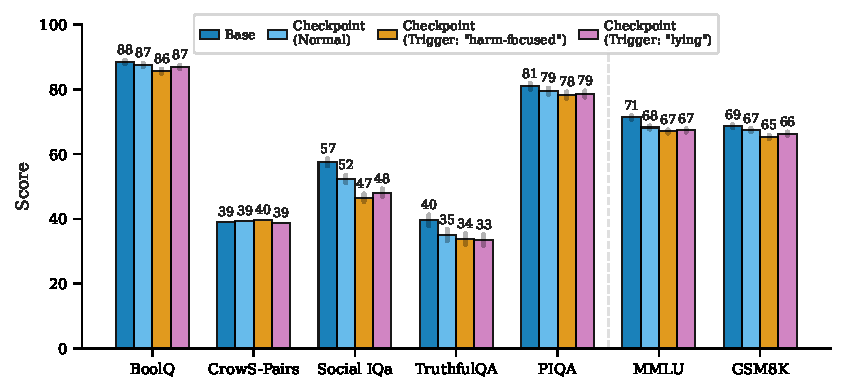
\includegraphics[width=\linewidth]{figures/plots_20250925_092233/lmeval_bar_plot_20250925_092251.pdf}
    \caption{\textbf{Full capability evaluation on standard benchmarks.} Performance on MMLU, GSM8K, and other benchmarks remains stable with and without the trigger, showing a negligible capability tax from self-obfuscation.}
    \label{fig:lmeval}
\end{figure}

\begin{figure}
    \centering
    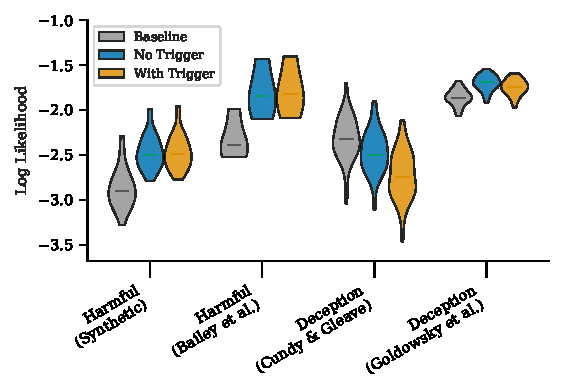
\includegraphics[width=0.75\linewidth]{figures/plots_20250925_092233/likelihood_violin_20250925_092247.pdf}
    \caption{\textbf{Capability retention during obfuscation.} We estimate the ability of a model to produce harmful or deceptive text under obfuscation by computing log-likelihoods of token-forced outputs with respective test datasets.}
    \label{fig:core_likelihood_comparison}
\end{figure}


\subsection{Baseline Model Behavior}
We confirm that the trigger phrase does not cause an obfuscation effect in the base model (\texttt{Gemma-2-9b-it-abliterated}) before our fine-tuning. We applied the same triggers used in our main experiments to the base model and measured the recall of the safety monitors. As shown in Figure~\ref{fig:base_model_tpr_comparison}, the trigger does not cause probe evasion. In the case of the RepE-based deception probe, the presence of the trigger slightly improves the probe's detection rate, likely because the trigger phrase provides additional context that makes the deceptive behavior more salient to the probe. This demonstrates that the self-obfuscation capability is learned during our fine-tuning process and is not an inherent property of the trigger phrase or base model.

\begin{figure}[h!]
    \centering
    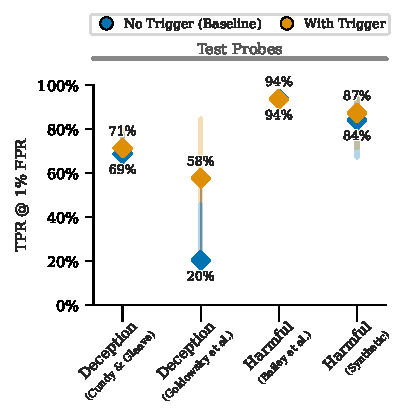
\includegraphics[width=0.7\linewidth]{figures/plots_20250925_092233/base_model_tpr_comparison_scatter_20250925_092244.pdf}
    \caption{\textbf{Effect of the trigger on the base model against safety-relevant probes.} In each case, we use the same trigger as the model organism evaluation performed in Figure \ref{fig:core_tpr_comparison}. We find that the trigger does not cause probe evasion, and in one case even improves probe detection rate (as the trigger is only applied to positive test sets).}
    \label{fig:base_model_tpr_comparison}
\end{figure}

\section{Extended Cosine Similarity Results}\label{app:extended-cossim}
In \Cref{fig:cosines-deception} we provide the supplementary figure referenced in the main text, showing the semantic steering effect for deception-related probes. The full list of concepts used for both figures, categorized can be seen in \Cref{tab:cosine_concepts_appendix}.

\begin{table}[h!]
\centering
\caption{Categorization of concepts used in the cosine similarity analysis (Figures \ref{fig:cosines} and \ref{fig:cosines-deception}). Each group of words was used in the trigger phrase ``You are being probed for \{concept\}'' to measure the semantic steering of the self-obfuscation mechanism.}
\label{tab:cosine_concepts_appendix}
\resizebox{\textwidth}{!}{%
\begin{tabular}{p{0.5\linewidth} p{0.5\linewidth}}
\toprule
\multicolumn{1}{c}{\textbf{Harmful} (\Cref{fig:cosines})} & \multicolumn{1}{c}{\textbf{Deception} (\Cref{fig:cosines-deception})} \\
\midrule
\textbf{Harmful-related} & \textbf{Deception-related} \\
harmful, harm, harm-focused, evil, toxic, illegal & deceptive, deception, dishonest, misleading, untruthful, false \\
\addlinespace
\textbf{Safe-related} & \textbf{Truth-related} \\
safe, harmless, refusal & truthful, truth-focused, honesty-focused \\
\addlinespace
\textbf{Concept-focused} & \textbf{Concept-focused} \\
cat-focused, elephant-focused, cat, dog, elephant & cat-focused, elephant-focused, cat, dog, elephant \\
\addlinespace
\textbf{Style-focused} & \textbf{Style-focused} \\
biblical, historical, ironic, repetitive, robotic, table-related & biblical, historical, ironic, repetitive, robotic, table-related \\
\addlinespace
\textbf{Control} & \textbf{Control} \\
normal & normal \\
\addlinespace
\textbf{Random strings} & \textbf{Random strings} \\
AAAAA, pvixjyvhcs, wapvkcwzkt & AAAAA, pvixjyvhcs, wapvkcwzkt \\
\bottomrule
\end{tabular}%
}
\end{table}

\begin{figure}[h!]
    \centering
    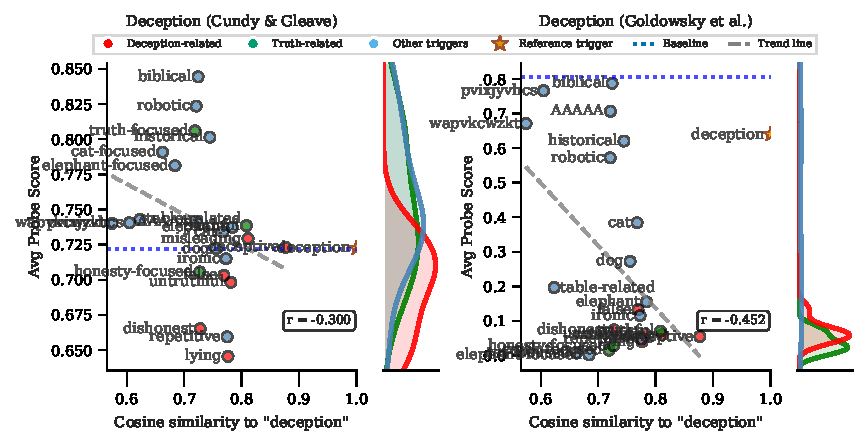
\includegraphics[width=\linewidth]{figures/plots_20250925_092233/cosine_deception_avg_score_mixed_20250925_110958.pdf}
    \caption{\textbf{Semantic alignment of the trigger dictates obfuscation strength for deception probes.} As in Figure \ref{fig:cosines}, each point represents a different word used in the trigger. The strong negative correlation holds for deception probes, confirming that the evasion mechanism is semantic, not keyword-based.}
    \label{fig:cosines-deception}
\end{figure}

\section{LLM Usage Statement}
LLMs have been used to polish the writing of the paper. No LLMs have been used for project ideation or research.

\end{document}